\documentclass[]{interact}
\usepackage[T1]{fontenc}
\usepackage[utf8]{inputenc}
\usepackage{booktabs,amsmath,amssymb,graphicx,url,placeins,enumitem,array,longtable,caption}
\providecommand{\tablebodyfont}{\small}
\providecommand{\tablefootnotefont}{\small}
\usepackage[mathlines]{lineno}
\renewcommand\linenumberfont{\normalfont\scriptsize\sffamily}
\setlength\linenumbersep{10pt}
\graphicspath{{./}{figures/}{figures/si/}}
\setlist[itemize]{leftmargin=1.5em,itemsep=2pt,topsep=3pt}
\setlength{\parskip}{1.5pt}
\raggedbottom
\renewcommand{\thefigure}{S\arabic{figure}}
\renewcommand{\thetable}{S\arabic{table}}
\begin{document}

% ==================================================================
% TITLE PAGE
% ==================================================================

\begin{center}
\vspace*{0.12\textheight}

{\fontsize{11}{14}\selectfont\bfseries
Supporting Information for\par}

\vspace{8pt}

{\fontsize{18}{22}\selectfont\bfseries
When Do Extreme-Demand Models Improve Tariff Decisions?
A Computational Comparison\par}

\vspace{14pt}

{\fontsize{10}{13}\selectfont
Mingyu Huang, Jiangweixi Wang, Zheng Gao, Yihang Yuan, and Zhengjun Yang\par}

\vspace{4pt}

{\fontsize{9}{12}\selectfont
Department of Statistics and Data Science, School of Mathematics and Statistics, Yunnan University, Kunming 650500, China\par}

\vspace{10pt}

{\fontsize{9}{12}\selectfont
Communications in Statistics -- Simulation and Computation\par}

{\fontsize{9}{12}\selectfont Correspondence: Mingyu Huang; \texttt{huangmingyu@stu.ynu.edu.cn}\par}

\end{center}

\vfill
\clearpage
\resetlinenumber[1]\linenumbers


% ==================================================================
% APPENDIX S1
% ==================================================================

\section*{Appendix S1. Supplementary methods, derivations, and analyses}

This Supporting Information provides technical derivations,
implementation details, complete supplementary summaries, robustness
analyses, and external predictive analyses referenced in the main
article. The primary controlled experiment compares five predictive
constructions. TAIL and EVENT-EMP use event-level histories, whereas
GEV, KDE, and EMP use the corresponding monthly maxima. The primary controlled
experiment contains 10,000 independent 24-month histories and nine
prespecified tariff cells, giving 450,000
history--method--cell decisions. Supplementary recovery, stress,
physical-clipping, and physical-misspecification experiments are
separate experiments and retain their own stated analysis units.

Throughout, \(M\geq0\) denotes monthly maximum demand,
\(F\) its distribution,
\[
\mu_F=\mathbb E_F[M],
\qquad
H_F(t)=\mathbb E_F[(M-t)_+].
\]
The reference capacity is \(S\), the contract level is \(D\),
the contract-threshold multiplier is \(\alpha\), the lower contract
fraction is \(\delta\), and the exceedance-charge multiplier is
\(\kappa\). Optimized mode values are denoted by \(V_F(m)\),
the oracle value by \(V_F^\ast\), oracle mode separation by
\(\gamma_F\), and the maximum mode-value perturbation by \(e_V\).
The retrospective stability ratio is
\[
d_{MV}=\frac{2e_V}{\gamma_F}.
\]
For a selected full action \(\widehat a\), regret is
\[
R_F(\widehat a)
=
C_F(\widehat a)-V_F^\ast.
\]


% ==================================================================
% S1.1
% ==================================================================

\subsection*{S1.1 Supplementary tariff identities and decision-stability details}

This subsection records the derivative, boundary, and proof details
underlying the contract-demand and mode-stability results in the main
article. The tariff cell and its feasible action set are fixed
throughout.

\paragraph*{Contract-demand optimization.}
For
\[
\phi_F(D)=D+\kappa H_F(\alpha D),
\qquad D\in\mathcal D_S=[\delta S,S],
\]
the stop-loss transform is finite, continuous, and convex. Its
one-sided derivatives are
\[
H'_{F,+}(t)=-\Pr_F(M>t),
\qquad
H'_{F,-}(t)=-\Pr_F(M\geq t).
\]
Thus, at an interior feasible $D$,
\[
\partial\phi_F(D)
=
\left[
1-\kappa\alpha\Pr_F(M\geq\alpha D),
\;
1-\kappa\alpha\Pr_F(M>\alpha D)
\right].
\]
The interior optimality condition is therefore
\[
\Pr_F(M>\alpha D^\ast)
\leq\frac{1}{\kappa\alpha}
\leq\Pr_F(M\geq\alpha D^\ast).
\]
When $\kappa\alpha>1$, this is equivalent to
\[
F(\alpha D^\ast-)\leq p^\ast\leq F(\alpha D^\ast),
\qquad
p^\ast=1-\frac{1}{\kappa\alpha}.
\]
This generalized-quantile condition allows atoms at the threshold. If
$F$ is continuous there, it reduces to $F(\alpha D^\ast)=p^\ast$.

For a nondegenerate feasible interval, convexity gives the following
boundary conditions:
\[
D^\ast=\delta S
\quad\Longleftrightarrow\quad
1-\kappa\alpha\Pr_F(M>\alpha\delta S)\geq0,
\]
and
\[
D^\ast=S
\quad\Longleftrightarrow\quad
1-\kappa\alpha\Pr_F(M\geq\alpha S)\leq0.
\]
When $\delta=1$, the feasible set is the singleton $\{S\}$. If
$\kappa\alpha<1$, the objective is strictly increasing on any
nondegenerate feasible interval and the lower boundary is the unique
optimizer. If $\kappa\alpha=1$, it is nondecreasing, so the lower
boundary is optimal and a flat interval may produce additional
minimizers.

For $\kappa\alpha>1$, set
\[
I_S=[\alpha\delta S,\alpha S],
\qquad
\operatorname{ES}_{p,I}(F)
=
\min_{t\in I}
\left\{
t+\frac{1}{1-p}\mathbb E_F[(M-t)_+]
\right\}.
\]
With $t=\alpha D$ and $1/(1-p^\ast)=\kappa\alpha$,
\[
D+\kappa H_F(\alpha D)
=
\frac{1}{\alpha}
\left\{
t+\frac{1}{1-p^\ast}H_F(t)
\right\}.
\]
Minimizing over the feasible interval gives
\[
V_F(\mathrm{con})
=
\frac{r_d}{\alpha}\operatorname{ES}_{p^\ast,I_S}(F).
\]
The unrestricted minimizer set of the variational objective is
\[
Q_{p^\ast}(F)
=
\{t\geq0:F(t-)\leq p^\ast\leq F(t)\}.
\]
If $Q_{p^\ast}(F)\cap I_S\neq\varnothing$, the constrained value
equals the ordinary Expected Shortfall scaled by $r_d/\alpha$, and the
optimal feasible thresholds are exactly this intersection. If the
sets do not intersect, convexity places the constrained minimizer at
the corresponding endpoint of $I_S$.

The exact within-contract loss identity follows by integrating the
almost-everywhere derivative of the stop-loss objective. For every
feasible $D$ and $D_F^\ast\in\mathcal D_F^\ast$,
\[
\phi_F(D)-\phi_F(D_F^\ast)
=
\int_{D_F^\ast}^{D}
\left[1-\kappa\alpha\{1-F(\alpha u)\}\right]\,du.
\]
For $\kappa\alpha>1$, writing $t=\alpha D$ and
$t_F^\ast=\alpha D_F^\ast$ gives
\[
C_F(a_{\mathrm{con}}(D))
-
C_F(a_{\mathrm{con}}(D_F^\ast))
=
r_d\kappa\int_{t_F^\ast}^{t}\{F(s)-p^\ast\}\,ds.
\]
The integral identity is unaffected by jumps in $F$. If $D_F^\ast$ is
interior and $F$ has a positive continuous density $f$ near
$t_F^\ast$, then $F(t_F^\ast)=p^\ast$ and
\[
C_F(a_{\mathrm{con}}(D))-C_F(a_{\mathrm{con}}(D_F^\ast))
=
\frac{r_d\kappa f(t_F^\ast)}{2}
(t-t_F^\ast)^2
+o\!\left((t-t_F^\ast)^2\right).
\]
This local quadratic expansion does not generally apply at a boundary
solution or an atom.

\paragraph*{Mode preservation and regret.}
For a unique oracle mode $m_F^\ast$, let
\[
\gamma_{F,m}=V_F(m)-V_F(m_F^\ast)>0,
\qquad
e_m=|V_{\widehat F}(m)-V_F(m)|.
\]
For each competitor,
\[
\begin{aligned}
V_{\widehat F}(m)-V_{\widehat F}(m_F^\ast)
&\geq V_F(m)-e_m-
\{V_F(m_F^\ast)+e_{m_F^\ast}\}\\
&=\gamma_{F,m}-e_m-e_{m_F^\ast}.
\end{aligned}
\]
Consequently, $e_m+e_{m_F^\ast}<\gamma_{F,m}$ for every competitor
implies preservation of the unique oracle mode. Uniform perturbation
of primitive-action costs by
\[
\varepsilon(F,\widehat F)
=
\sup_{a\in\mathcal A_S}
|C_{\widehat F}(a)-C_F(a)|
\]
implies
\[
e_m\leq\varepsilon(F,\widehat F)
\quad\text{for every }m\in\mathcal M.
\]
For the contract mode this follows from the standard inequality
bounding the difference between two minima by the uniform difference
between their objectives. Hence
$\gamma_F>2\varepsilon(F,\widehat F)$, where
$\gamma_F=\min_{m\neq m_F^\ast}\gamma_{F,m}$, implies all pairwise
conditions.

The scalar condition uses
\[
e_V=\max_{m\in\mathcal M}e_m,
\qquad
d_{MV}=\frac{2e_V}{\gamma_F}.
\]
If $d_{MV}<1$, then for every competitor
\[
e_m+e_{m_F^\ast}
\leq2e_V<\gamma_F\leq\gamma_{F,m},
\]
so the pairwise condition applies. When the oracle minimum is not
unique, stability is formulated by excluding positive-gap nonoptimal
modes; it does not preserve an arbitrary label among tied oracle
minimizers.

For an exact fitted-optimal action, the regret bound follows from
optimality under $\widehat F$ and the uniform primitive-action
perturbation:
\[
0\leq R_F(\widehat a)\leq2\varepsilon(F,\widehat F).
\]
The exact decomposition into mode-selection loss and within-mode
excess is algebraic. The within-mode excess is zero for actual-demand
and capacity actions because their feasible sets are singletons. If
contract demand is selected and oracle-optimal and $\widehat D$
minimizes the fitted contract objective, then
\[
0\leq R_F(a_{\mathrm{con}}(\widehat D))
\leq2r_d\kappa\Delta_H(F,\widehat F),
\qquad
\Delta_H(F,\widehat F)
=
\sup_{D\in\mathcal D_S}
|H_{\widehat F}(\alpha D)-H_F(\alpha D)|.
\]
For an approximate fitted action with objective suboptimality at most
$\zeta$, the general bound becomes
$R_F(\widetilde a)\leq2\varepsilon(F,\widehat F)+\zeta$.

\paragraph*{Wasserstein mode-stability bounds.}
For nonnegative distributions with finite first moments,
\[
W_1(F,G)=\int_0^\infty|F(x)-G(x)|\,dx
\]
bounds both the mean difference and every stop-loss difference:
\[
|\mu_G-\mu_F|\leq W_1(F,G),
\qquad
|H_G(t)-H_F(t)|\leq W_1(F,G).
\]
The mode-value perturbation constants are
\[
L_{\mathrm{cap}}=0,\qquad
L_{\mathrm{act}}=r_d,\qquad
L_{\mathrm{con}}=r_d\kappa.
\]
The contract bound follows because the two contract objectives differ
uniformly over the common feasible set by at most
$r_d\kappa W_1(F,G)$; the difference between their minima is no larger
than this uniform difference.

For capacity--actual and capacity--contract contrasts, the direct
constants follow from the preceding mode-value bounds. For the
actual--contract contrast, define
\[
g_D(x)=x-D-\kappa(x-\alpha D)_+.
\]
Then
\[
V_F(\mathrm{act})-V_F(\mathrm{con})
=
r_d\sup_{D\in\mathcal D_S}\mathbb E_F[g_D(M)].
\]
The slopes of $g_D$ are $1$ and $1-\kappa$, so
$\operatorname{Lip}(g_D)=\max\{1,|1-\kappa|\}$ uniformly in $D$.
By the Kantorovich--Rubinstein inequality,
\[
\left|
\mathbb E_G[g_D(M)]-\mathbb E_F[g_D(M)]
\right|
\leq
\max\{1,|1-\kappa|\}W_1(F,G).
\]
Taking suprema over the same feasible set proves
\[
|\Delta_{G,\mathrm{act},\mathrm{con}}
-\Delta_{F,\mathrm{act},\mathrm{con}}|
\leq
r_d\max\{1,|1-\kappa|\}W_1(F,G).
\]
Thus the direct pair constants are
\[
K_{\mathrm{cap},\mathrm{act}}=r_d,\qquad
K_{\mathrm{cap},\mathrm{con}}=r_d\kappa,\qquad
K_{\mathrm{act},\mathrm{con}}
=r_d\max\{1,|1-\kappa|\}.
\]
If the oracle mode is unique, a sufficient direct-contrast radius is
\[
\rho_F^{\mathrm{contrast}}
=
\min_{m\neq m_F^\ast}
\frac{\gamma_{F,m}}{K_{m,m_F^\ast}}.
\]
Indeed, the contrast between any competitor and the oracle mode stays
positive whenever $K_{m,m_F^\ast}W_1(F,G)<\gamma_{F,m}$ for every
competitor.

Bounding each mode separately gives the mode-wise pairwise radius
\[
\rho_F^{\mathrm{pair}}
=
\min_{m\neq m_F^\ast}
\frac{\gamma_{F,m}}{L_m+L_{m_F^\ast}},
\]
while $L=r_d\max\{1,\kappa\}$ gives the uniform radius
\[
\rho_F=\frac{\gamma_F}{2L}.
\]
The direct constants equal the sums of mode constants for comparisons
involving capacity. For actual versus contract demand,
\[
r_d\max\{1,|1-\kappa|\}
\leq r_d(1+\kappa),
\]
so the direct contrast constant is no larger than the corresponding
mode-wise sum. Also $L_m+L_{m_F^\ast}\leq2L$ and
$\gamma_{F,m}\geq\gamma_F$. Therefore
\[
\rho_F^{\mathrm{contrast}}
\geq\rho_F^{\mathrm{pair}}
\geq\rho_F.
\]
The radii are expressed in the same demand units as $M$; in the
controlled experiment, these units are kW. The uniform perturbation
bound also gives
\[
\varepsilon(F,G)\leq LW_1(F,G),
\qquad
R_F(\widehat a)\leq LW_1(F,\widehat F)
\]
for an exact fitted-optimal action. For any two feasible primitive
actions $a,b$, the realized cost difference $c(x,a)-c(x,b)$ is
$L$-Lipschitz because every primitive-action cost is nondecreasing
with slope in $[0,L]$. If $a_F$ minimizes cost under $F$ and
$\widehat a$ minimizes under $\widehat F$, then
$\mathbb E_{\widehat F}[c(M,\widehat a)-c(M,a_F)]\leq0$.
Applying the Kantorovich--Rubinstein inequality to this action
contrast gives the displayed regret bound. A fitted optimization
gap $\zeta$ adds $\zeta$ to the right-hand side.

As an implementation check, the exact regret decomposition was
verified on all $450{,}000$ primary decision rows, with no failures;
the maximum absolute residual was
$7.45\times10^{-9}$ CNY/month.

\subsection*{S1.2 Analytic oracle and deterministic numerical evaluation}

The controlled data-generating mechanism admits an analytic
monthly-maximum distribution. In each month, 200 bounded bulk events
are generated as
\[
X^{(b)}
=
45{,}000+35{,}000\,B,
\qquad
B\sim\operatorname{Beta}(8,2),
\]
and an independent number
\[
N\sim\operatorname{Poisson}(30)
\]
of tail events is generated as
\[
X^{(t)}
=
80{,}000+Y,
\qquad
Y\sim\operatorname{GPD}(\xi=0.15,\sigma=12{,}000).
\]
The monthly maximum \(M\) is the maximum over the bulk and tail
events.

Let
\[
L=45{,}000,
\qquad
u_0=80{,}000,
\qquad
\lambda=30,
\]
and let \(F_B\) denote the
\(\operatorname{Beta}(8,2)\) distribution function. The exact
monthly-maximum CDF is
\[
F_M(x)
=
\begin{cases}
0,
&
x<L,
\\[4pt]
\exp(-\lambda)
\left[
F_B\!\left(
\dfrac{x-L}{u_0-L}
\right)
\right]^{200},
&
L\leq x<u_0,
\\[10pt]
\displaystyle
\exp\left[
-\lambda
\left\{
1+\xi\frac{x-u_0}{\sigma}
\right\}^{-1/\xi}
\right],
&
x\geq u_0.
\end{cases}
\]

The resulting oracle quantities are
\[
\mu_F
=
148{,}235.371489\ {\rm kW},
\]
\[
q_{0.99}
=
265{,}663.010007\ {\rm kW},
\]
and
\[
q_{0.999}
=
375{,}513.529996\ {\rm kW}.
\]

The oracle mean and stop-loss functionals are evaluated from
\[
\mu_F
=
\int_0^\infty
\{1-F_M(x)\}\,dx
\]
and
\[
H_F(t)
=
\int_t^\infty
\{1-F_M(x)\}\,dx.
\]
High quantiles are obtained from the analytic distribution. The same
oracle law therefore determines the reference capacity
\[
S=\frac{\mu_F}{u},
\]
the tariff-mode values, the optimized contract level, the unique
oracle mode where applicable, and the oracle mode separation
\(\gamma_F\).

Final fitted-law evaluation likewise avoids a common predictive
Monte Carlo layer between \(\widehat F\) and the tariff functionals.
Finite discrete distributions use exact sums. The nonnegative
Gaussian KDE uses analytic Gaussian-mixture expressions for its mean
and stop-loss function. The fitted tail-process and
nonnegative-conditioned GEV constructions use deterministic
one-dimensional integration where required, and continuous quantiles
are obtained by direct inversion or deterministic bracketed root
finding.

The deterministic numerical layer was independently checked in
55 numerical comparisons. The maximum relative discrepancy was
approximately
\[
1.283\times10^{-11}.
\]
No Monte Carlo approximation to the oracle is used in the reported
controlled experiment.


% ==================================================================
% S1.3
% ==================================================================

\subsection*{S1.3 Predictive-construction implementation}

The five primary predictive constructions are organized by their
information source. TAIL and EVENT-EMP use event-level observations.
GEV, KDE, and EMP use the 24 observed monthly maxima. This distinction
is retained because comparisons across the two groups combine
differences in information resolution and distributional construction,
whereas TAIL versus EVENT-EMP and comparisons within
GEV/KDE/EMP provide same-broad-information contrasts.


\subsubsection*{Event-level constructions}

\paragraph*{TAIL.}

TAIL receives event-level maxima with month identifiers. Candidate
threshold quantiles are $0.90,0.925,0.95,0.975$. For each 24-month
history, the months form four disjoint validation folds of six months.
For each candidate quantile and fold, the threshold and model are estimated
from the other 18 months. Strict event exceedances $Z>u$ have GPD excess
law $Y=Z-u$, fitted by maximum likelihood with location fixed at zero.

Monthly exceedance counts include months with zero exceedances. If the
variance-to-mean ratio is at most 1.2, the count law is Poisson; otherwise
the negative-binomial method-of-moments parameters are
\[
r=\frac{\bar N^2}{s_N^2-\bar N},\qquad p=\frac{r}{r+\bar N}.
\]
The empirical maximum of subthreshold events within each fitting month
provides the subthreshold component. A candidate fold requires at least
100 strict excesses and a finite-mean fitted GPD with $\widehat\xi<1$.
The fitted monthly-maximum CDF is scored on each held-out maximum by
\[
\operatorname{CRPS}(F,y)
=\int_0^y F(x)^2\,dx+\int_y^\infty\{1-F(x)\}^2\,dx.
\]
The first integral uses the empirical subthreshold steps exactly; the
tail integrals use deterministic adaptive quadrature. The score for a
candidate is the mean of its 24 held-out CRPS values, and the lowest
score selects the quantile. Exact ties favour the lower quantile.

After selection, the numerical threshold is recomputed from all 24
months and the GPD, count model, and subthreshold component are refitted.
The selected full-history GPD fit receives a 500-resample nonparametric
shape bootstrap. At least 400 successful refits are required and the
95\% shape-interval width must be at most 0.8. If $\widehat\xi<0$,
its endpoint $u-\widehat\sigma/\widehat\xi$ must cover all observed
event maxima. No same-sample nominal KS $p$-value or shape penalty is
used to select a threshold.

The four-fold selector requires at least one complete finite-mean
candidate across the four folds. After a threshold has been selected,
the full-history fit is checked for finite mean, observed-support
compatibility, and the prespecified shape-width gate. If the selected
full-history fit fails a final gate and at least 50 exceedances are
available, the procedure uses an exponential tail with $\xi=0$ and
scale equal to the mean excess. If this fallback is unavailable, it
uses the empirical distribution of monthly maxima. Every primary
history in the reported run had a complete
finite-mean candidate and a valid final fit.

For a final primary TAIL fit, let \(F_0\) denote the empirical CDF of
the subthreshold monthly-maximum component, let \(G_u\) denote the
fitted GPD excess CDF, and let \(P_N\) denote the fitted exceedance-count
probability-generating function. The monthly-maximum CDF is
\[
\widehat F_{\rm TAIL}(x)
=
\begin{cases}
F_0(x)P_N(0),
&
x<u,
\\[4pt]
P_N\!\left\{G_u(x-u)\right\},
&
x\geq u.
\end{cases}
\]
The final mean is evaluated as
\[
\mu_{\widehat F_{\rm TAIL}}
=
H_{\widehat F_{\rm TAIL}}(0),
\]
the stop-loss function is obtained by deterministic integration of the
fitted survival function, and continuous quantiles are obtained by
deterministic inversion. The deterministic held-out CRPS used for threshold selection is
separate from evaluation of the final tariff-relevant functionals.



\paragraph*{EVENT-EMP.}

EVENT-EMP uses the same event-level history as TAIL but imposes no
threshold or parametric tail/count model. Let \(\widehat G_E\) denote
the pooled empirical CDF of all event-level maxima in the 24-month
history, and let \(N_m\) denote the observed total event count in
month \(m\). The induced monthly-maximum CDF is
\[
\widehat F_{\rm EE}(x)
=
\frac{1}{24}
\sum_{m=1}^{24}
\widehat G_E(x)^{N_m}.
\]
This is a finite discrete distribution. Its probability masses are the
jumps of \(\widehat F_{\rm EE}\); its mean and stop-loss function are
evaluated exactly by finite sums, and its quantiles use the discrete
left inverse. There is no dedicated fallback branch.

TAIL and EVENT-EMP therefore use the same broad event-level
information source but different distributional constructions. TAIL
adds threshold selection, a parametric excess law and a fitted
exceedance-count law, whereas EVENT-EMP combines a pooled empirical
event distribution with the empirical distribution of observed
monthly event counts.


\subsubsection*{Monthly-maxima constructions}

\paragraph*{GEV.}

The controlled-experiment GEV construction uses the 24 observed
monthly maxima. It is fitted using L-moments/probability-weighted
moments rather than maximum likelihood. L-skewness is inverted
deterministically for the EVT shape parameter within
\[
[-0.90,0.90],
\]
and the location and scale parameters follow from the associated
L-moment equations.

A successful raw GEV fit is conditioned on the nonnegative part of its
model-implied natural support. If more than 1\% of the raw fitted GEV
probability lies below zero, or if the L-moment fit or resulting
parameters are invalid, the procedure uses the empirical
monthly-maxima distribution. Successful parametric fits satisfy the
finite-mean requirement. When the fitted EVT shape is negative, its
model-implied finite upper endpoint is retained; otherwise the upper
support is unbounded.

The conditioned GEV mean and stop-loss function are evaluated
deterministically over this support, using one-dimensional integration
where required. Quantiles use the conditioned inverse distribution.
This GEV construction is distinct from the K-GEV procedure used in the
external manufacturing-load analysis.


\paragraph*{KDE.}

KDE is fitted to the 24 monthly maxima
\(M_1,\ldots,M_n\), with \(n=24\), using bandwidth
\[
h
=
1.06\,s\,n^{-1/5},
\]
where \(s\) is the sample standard deviation. The Gaussian mixture is
conditioned on nonnegative demand. If
\[
\widetilde F(x)
=
\frac{1}{n}
\sum_{i=1}^{n}
\Phi\left(\frac{x-M_i}{h}\right)
\]
denotes the unconditioned Gaussian-mixture CDF and
\[
Z_+
=
1-\widetilde F(0),
\]
then
\[
\widehat F_{\rm KDE}(x)
=
\begin{cases}
0,
&
x<0,
\\[3pt]
\dfrac{\widetilde F(x)-\widetilde F(0)}{Z_+},
&
x\geq0.
\end{cases}
\]

For \(t\geq0\), its stop-loss function is
\[
H_{\widehat F_{\rm KDE}}(t)
=
\frac{1}{nZ_+}
\sum_{i=1}^{n}
\left[
(M_i-t)
\Phi\left(\frac{M_i-t}{h}\right)
+
h\phi\left(\frac{t-M_i}{h}\right)
\right],
\]
where \(\Phi\) and \(\phi\) are the standard normal CDF and PDF.
Setting \(t=0\) gives the mean. Quantiles are obtained by deterministic
inversion of the conditioned mixture CDF. If fewer than two
observations are available or the observed variability is numerically
degenerate, the implementation uses the empirical distribution.


\paragraph*{EMP.}

EMP assigns empirical probability to the 24 observed monthly maxima,
with duplicate support values aggregated. For support points \(x_j\)
with empirical probabilities \(p_j\),
\[
\mu_{\widehat F_{\rm EMP}}
=
\sum_jp_jx_j,
\]
and
\[
H_{\widehat F_{\rm EMP}}(t)
=
\sum_jp_j(x_j-t)_+.
\]
Quantiles use the empirical left inverse. No predictive-bootstrap layer
is introduced into the final tariff-functional evaluation.


% ==================================================================
% S1.4
% ==================================================================

\subsection*{S1.4 From predictive laws to tariff actions}

Every fitted predictive law is passed through the same tariff-action
map. For the evaluated policies, \(\kappa\alpha>1\), and the interior
contract probability is
\[
p^\ast
=
1-\frac{1}{\kappa\alpha}.
\]
For a fitted law \(\widehat F\), define the left generalized quantile
\[
\widehat q_p
=
\inf\{x:\widehat F(x)\geq p\}.
\]
The final contract level is
\[
\widehat D
=
\operatorname{clip}
\left(
\frac{\widehat q_{p^\ast}}{\alpha},
\delta S,
S
\right).
\]
Thus lower and upper boundary solutions are handled directly through
the feasible interval. No predictive Monte Carlo candidate search or
local order-statistic candidate set is used.

The fitted optimized tariff-mode values are
\[
V_{\widehat F}(\operatorname{cap})
=
r_cS,
\]
\[
V_{\widehat F}(\operatorname{act})
=
r_d\mu_{\widehat F},
\]
and
\[
V_{\widehat F}(\operatorname{con})
=
r_d
\left\{
\widehat D
+
\kappa
H_{\widehat F}(\alpha\widehat D)
\right\}.
\]
The selected tariff mode minimizes these deterministic mode values.
Exact mode-value ties are resolved by the fixed lexicographic order
\[
\operatorname{actual\ demand}
\;\prec\;
\operatorname{capacity}
\;\prec\;
\operatorname{contract\ demand}.
\]

For discrete predictive laws, the left-quantile convention fixes the
generalized-quantile representative. For continuous laws, quantiles
are obtained directly or by deterministic root inversion.

Although
\[
V_F(\operatorname{cap})=r_cS
\]
does not itself contain a distributional functional, selection of the
capacity mode depends on its comparison with the estimated
actual-demand and contract-demand mode values. Under contract demand,
the complete action additionally contains \(D\); consequently,
tariff-mode correctness and full-action optimality are separate
endpoints.


% ==================================================================
% S1.5
% ==================================================================

% ==================================================================
% S1.5
% ==================================================================

\subsection*{S1.5 Primary comparisons and high-$p^*$ tariff stress}

The main article reports the nine-cell primary summaries and the
mode-versus-within-contract regret decomposition. Table~\ref{tab:final-si-11} gives all ten
history-paired regional method contrasts. The high-$p^*$ stress uses
10,000 histories, five methods, and ten utilization cells at each of
three target levels; Figure~\ref{fig:final-figures1} and
Table~\ref{tab:si-high-pstar} report its mean regret by utilization
cell, exact-zero-regret rates, and paired regional comparisons.
With $\alpha=2.20$, the target levels $p^*=0.90$, $0.95$, and $0.99$
correspond to penalty multipliers $\kappa\approx4.545$, $9.091$, and
$45.455$, respectively. The oracle contract-demand regions contain
eight, seven, and four of the ten utilization cells at these target
levels. Regional contrasts are equal-weight averages over the cells in
each target-specific oracle region and therefore describe tariff
configurations with different penalty scales and oracle-region
compositions.

% ==================================================================
% S1.6
% ==================================================================

\subsection*{S1.6 Functional-error associations and stability-conditioned loss}

Figure~\ref{fig:final-figures2} summarizes the within-method association
of regret with absolute mean, stop-loss, and $q_{0.99}$ relative errors,
and the concentration of regret among the largest-loss decisions.
Table~\ref{tab:final-si-7} reports the paired functional-correlation
contrasts with simultaneous max-$|T|$ intervals.
Table~\ref{tab:si-stability-condition} reports within-contract loss
among decisions stratified by whether each mode-stability condition is
satisfied.

% ==================================================================
% S1.7
% ==================================================================

\subsection*{S1.7 Numerical bounds}

The theoretical sufficient conditions in the main article are
summarized separately from their numerical implementation. The
numerical implementation checks combine upper constructions for the
distributional perturbations with a common full-action solver allowance.
For the primitive-action perturbation, the reported numerical upper
quantity is
\[
\varepsilon_{\rm num}
=\max\left\{
r_d\left|\widehat\mu-\mu_F\right|,
\;r_d\kappa\Delta_{H,\rm upper}
\right\}.
\]
It is a numerical upper bound on primitive-action perturbation, not the
mode-value error $e_V$ and not an exact analytic supremum. The
feasible-threshold stop-loss quantity uses a direct 513-node estimate
and a numerical upper allowance based on the monotone-CDF envelope and
half-grid spacing; it is a numerical upper bound on the feasible
stop-loss perturbation.

The primitive numerical sufficient-condition check is
\[
2\varepsilon_{\rm num}+\zeta_{\rm full,num}<\gamma_F.
\]
For each non-oracle competitor $m$, the direct
contrast-Wasserstein check is
\[
K_{m,m_F^\ast}W_{1,\rm upper}
+\zeta_{\rm full,num}<\gamma_{F,m},
\]
where $K_{\mathrm{cap},\mathrm{act}}=r_d$,
$K_{\mathrm{cap},\mathrm{con}}=r_d\kappa$, and
$K_{\mathrm{act},\mathrm{con}}=r_d\max\{1,|1-\kappa|\}$.
The mode-wise pairwise Wasserstein comparator instead uses
\[
(L_m+L_{m_F^\ast})W_{1,\rm upper}
+\zeta_{\rm full,num}<\gamma_{F,m},
\]
for every non-oracle competitor, and the uniform Wasserstein check is
\[
2L W_{1,\rm upper}+\zeta_{\rm full,num}<\gamma_F,
\qquad L=r_d\max\{1,\kappa\}.
\]
The adaptive numerical Wasserstein bracket integrates the CDF
difference on a nonuniform log-demand grid, refines the intervals with
the largest uncertainty, and adds an analytic right-tail allowance.
We intersected the adaptive bracket with the archived monotone-CDF
bracket. The reported checks use the upper endpoint of this
intersection. The 300 kW width target applies to the adaptive bracket.
The full-action regret comparison permits the uniform check
\[LW_{1,\rm upper}+\zeta_{\rm full,num}<\gamma_F.\]
The preceding $2L$ condition remains a valid mode-value comparator;
Table~\ref{tab:numerical-sufficient-condition-audit} reports the
full-action regret check. Across 50,000 fitted laws, 49,936 adaptive
brackets had width at most 300 kW. The GEV median bracket width was
260.972 kW, its 95th percentile was 296.453 kW, and its 99th
percentile was 299.634 kW. Table~S6 reports
method-level brackets and Figure~S3 shows the revised checks.
The primitive check passed in $24{,}894/450{,}000$ decisions
($5.532\%$), the direct contrast check in $59{,}410$ ($13.202\%$),
the per-competitor mode-wise check in $27{,}352$ ($6.078\%$), and the
full-action regret check in $31{,}677$ ($7.039\%$). No observed mode
errors occurred among passing rows. The known generating law supplies
these simulation diagnostics.
For the full-action regret condition, $31{,}677$ decisions satisfy the
condition using the numerical $W_1$ upper bound, $415{,}130$ cannot
satisfy it even at the lower bound, and $3{,}193$ ($0.710\%$) remain
undetermined by the integration bracket. All undetermined rows have
bracket widths below 300 kW. These are classifications of the
sufficient-condition calculation, separate from observed mode errors.

\subsection*{S1.8 Parameter recovery and threshold-fixed bootstrap interval coverage}


The parameter-recovery experiment is separate from the 10,000-history
primary comparison. It uses 200 histories at each of 12, 24, and
60 months under a Poisson--GPD mechanism with generating threshold
\(80{,}000\) kW,
\[
\xi=0.15,
\qquad
\sigma=12{,}000\ {\rm kW},
\]
and a Poisson rate of 30 tail events per month.

The threshold continues to be selected by the fitted procedure rather
than fixed at the generating threshold. Scale recovery is therefore
evaluated relative to the threshold-specific scale implied by GPD
threshold stability.

The mean absolute errors of the fitted shape parameter are
\[
0.0699,\qquad
0.0578,\qquad
0.0343
\]
for 12, 24, and 60 months, respectively. Figure S4 reports the
complete shape-error, relative-scale-error, and relative-\(q_{0.99}\)
error distributions.

\FloatBarrier

For each history of length \(n\) months, we construct nominal 95\%
nonparametric percentile intervals for the GPD shape and scale.
The selected threshold \(\widehat v\) is held fixed. We draw 100
bootstrap samples with replacement from the excesses in the first
\(\lfloor0.8n\rfloor\) months, preserving the excess count, and fit
a GPD with location fixed at zero to each sample. The interval
endpoints are the 2.5th and 97.5th percentiles of the valid parameter
estimates; at least 75 finite fits with positive scale are required.
Shape coverage is evaluated against \(\xi=0.15\), and scale coverage
against \(\sigma(\widehat v)=12000+0.15(\widehat v-80000)\).
Table~S10 reports coverage across 200 histories and 95\%
Clopper--Pearson intervals for its Monte Carlo uncertainty.
Thresholds vary across histories and remain fixed within each
bootstrap calculation.


% ==================================================================
% S1.9
% ==================================================================

\subsection*{S1.9 Physical clipping identity and sensitivity}

Let latent event-level demand values be \(X_i\), and let physical
clipping operate at level \(c\). Clipping commutes with maximization:
\[
\min\left(\max_iX_i,c\right)
=
\max_i\min(X_i,c).
\]
Thus clipping individual events before monthly maximization yields the
same clipped monthly maximum as clipping the corresponding original
monthly maximum.

Let
\[
M_c=\min(M,c)
\]
and let \(F_c\) denote its distribution. Pointwise,
\[
M_c=M-(M-c)_+,
\]
so
\[
\mathbb E[M_c]
=
\mathbb E[M]-H_F(c).
\]
For every \(t\leq c\),
\[
(\min(M,c)-t)_+
=
(M-t)_+-(M-c)_+,
\]
and therefore
\[
H_{F_c}(t)
=
H_F(t)-H_F(c),
\qquad
t\leq c.
\]
For \(t\geq c\),
\[
H_{F_c}(t)=0.
\]
The equality case \(t=c\) is included in the first identity.

The clipping experiment uses four physical regimes:
\[
\begin{aligned}
\mathrm{UNCAPPED}:&
\quad c=10q_{0.999},
\\
\mathrm{DISTANT}:&
\quad c=\frac{q_{0.999}}{0.85},
\\
\mathrm{Q999}:&
\quad c=q_{0.999},
\\
\mathrm{BINDING}:&
\quad c=\frac{q_{0.999}}{1.25}.
\end{aligned}
\]
``UNCAPPED'' is an experimental label for a distant finite physical
clipping level. Its value \(c=10q_{0.999}\) defines a clipping regime
only in this robustness experiment. The clipping level \(c\) is
applied to generated demand and is distinct from the fitted-law support
treatment used in the primary controlled analysis.

The experiment uses 12- and 24-month histories,
\[
u\in\{0.62,0.63,0.64\},
\]
and 200 histories for each
history-length--clipping--utilization setting. TAIL, KDE, EMP, and the
robustness-only GATE selector are retained. In this experiment, normalized regret is one-month regret divided by
one monthly capacity fee;
it is distinct from the primary normalized regret \(R_F/V_F^\ast\).

GATE selects TAIL when its fit status is \texttt{PASS}, the fraction
of reconstructed maxima exceeding the support bound is at most 0.01,
and two consecutive available threshold candidates pass screening
with shape estimates of the same sign. Candidates are ordered by
their threshold quantiles \(0.90,0.925,0.95,0.975\); the qualifying
pair need not include the threshold ultimately selected by TAIL.
Each member must have at least 100 exceedances, a nominal 95\%
bootstrap shape-interval width at most 0.8, a uniform-transform KS
\(p\)-value at least 0.01, and an endpoint compatible with the clipping level when its
shape is negative. GATE otherwise selects KDE.
Shape-width screening uses 50 bootstrap resamples here and 500 in
the physical-pipeline experiment in S1.10, with at least 80\% valid refits.
The support bound is the clipping level \(c\) here and 120 MW in
S1.10. Two zero shape estimates count as having the same sign.

Figure S5 reports paired TAIL-minus-baseline ECDFs after averaging the
three utilization cells within history. Negative values favour TAIL.
ECDFs are used because the interquartile ranges of all 16 plotted
contrast groups are zero and boxplots would obscure their nonzero
tails.

\FloatBarrier



% ==================================================================
% S1.10
% ==================================================================

\subsection*{S1.10 Physical-pipeline stress at $\alpha=1.20$}

\paragraph*{Load-generating process.}
This separate stress protocol uses the fitting rule specified below.
The physical-pipeline scenarios are synthetic one-minute simulations of
an 80-ton electric arc furnace (EAF) and a background load. The EAF has
an 80-MW active-power cap and a target production rate of 5,000 heats
per year. Time to tap follows a normal distribution truncated to
60--70 minutes (mean 65 minutes, standard deviation 3 minutes); idle
time follows a gamma distribution with shape 4 and mean 40.12 minutes.
Each heat has six ordered stages. Their duration shares are drawn from
a Dirichlet distribution with concentration 80 and center
$(0.08,0.08,0.48,0.16,0.12,0.08)$; nominal stage powers are the
corresponding fractions $(0.03,0.05,0.75,0.50,0.40,0.05)$ of 80 MW.
Heat energy follows a lognormal distribution truncated to 32--58 MWh,
with mean 40 MWh and coefficient of variation 0.08. Within-stage power
deviations follow an AR(1) process with coefficient 0.85 and innovation
standard deviation 0.05 times nominal stage power. The resulting
profile is rescaled to the sampled heat energy, subject to the 80-MW
power cap.

Background demand has mean 20 MW and a 4-MW daily cosine component
peaking at 15:00. Its AR(1) component has coefficient 0.95 and
innovation standard deviation 1.5 MW; total background power is bounded
between 8 and 36 MW. Point-of-connection power is the sum of EAF and
background power. The simulated calendar has 30 days per month and
continuous operation. Monthly maxima are calculated from non-overlapping
15-minute averages of the one-minute point-of-connection series.

\paragraph*{Rare-event mechanisms.}
Each synthetic month first draws a Poisson number of rare-event
clusters. Cluster anchors are sampled without replacement from the
scheduled heats; the heat immediately following an anchor is assigned
to the same cluster with the scenario-specific probability below.
For each affected heat, a contiguous 8-minute segment is selected
uniformly within the melting stage. Its power increment is the
scenario's headroom fraction times a $\operatorname{Beta}(2,2)$ severity
draw times the remaining headroom to 80 MW. Power is capped at 80 MW,
and the added energy is limited so that a heat does not exceed 60 MWh.
The consecutive-heat event is a restart proxy within the next melting
stage, not a separate measured furnace state.

\[
\begin{array}{lccc}
\text{Scenario} & \text{Clusters/month} &
\text{Headroom} & \text{Consecutive probability}\\
\text{T4 high amplitude} & 1.0 & 0.75 & 0.30\\
\text{T5 high frequency} & 2.0 & 0.75 & 0.30\\
\text{T6 clustered events} & 2.0 & 0.75 & 0.60
\end{array}
\]
The headroom fraction and severity family are common to the three
scenarios; T4--T6 vary the event rate and the probability of a
consecutive affected heat.

\paragraph*{Training design and tariff cells.}
For each mechanism, the fixed truth library contains 5,000 training
months and a separate 20,000-month test pool. Each of 200 paired
replications samples 24 training months without replacement from the
training pool; the 12-month history is the first 12 months of that
same sampled history. Methods therefore use matched histories at both
training lengths. The 14 utilization levels are
\[
\begin{aligned}u\in\{&0.300,0.350,0.375,0.400,0.425,0.450,0.475,\\
&0.500,0.550,0.600,0.625,0.650,0.700,0.750\}.\end{aligned}
\]
All cells use $\alpha=1.20$, $\kappa=2$, $\delta=0.40$,
$r_d=36\,\mathrm{CNY/(kW\cdot month)}$, and
$r_c=22.5\,\mathrm{CNY/(kW\cdot month)}$. The synthetic tariff
calculations use the active-power scale throughout. For scenario $s$,
the frozen reference capacity is $S_{s,u}=\bar M_s/u$ kW, where
$\bar M_s$ is the mean fixed-15-minute monthly maximum in that
scenario's 20,000-month test pool. The three values of $\bar M_s$ for
T4, T5, and T6 are 101,866.243, 101,871.336, and 101,873.150 kW,
respectively. The same frozen capacity is used by every predictive
method in a scenario--utilization cell.

\paragraph*{Predictive constructions and oracle.}
EMP-JOINT resamples the training monthly maxima with replacement.
KDE-MC-JOINT uses an equally weighted Gaussian kernel mixture centered
at the training monthly maxima, with bandwidth $1.06s n^{-1/5}$, where
$s$ is the sample standard deviation and $n$ is the training length.
Predictive draws are generated by resampling a training maximum and
adding Gaussian noise with this bandwidth; proposals below zero are
rejected. TAIL-JOINT fits a process-aware peaks-over-threshold
model to heat-level maxima, grouping records from the same rare-event
cluster and retaining nonclustered heats as separate events. Candidate
thresholds are the empirical 0.90, 0.925, 0.95, and 0.975 quantiles of fitting-period process-event maxima.
Exceedances follow a generalized Pareto distribution, while monthly
exceedance counts use a Poisson model unless their variance-to-mean
ratio exceeds 1.2, in which case a negative-binomial model is used.
The last 20\% of training months are reserved for validation. Candidate
fits require at least 100 exceedances, a bootstrap 95\% shape-interval
width no greater than 0.8, and a nominal probability-transform KS $p$-value of at least 0.01.
This legacy screen is a fit diagnostic; its nominal $p$-value
is not calibrated for GPD parameters fitted to the same excesses. For a negative-shape candidate, its finite endpoint must
be no lower than the observed maximum and no higher than the
120,000-kW physical bound. Five hundred bootstrap refits are used for
the shape-width check. The selected candidate maximizes the
validation log score with a 0.10 penalty on deviation of its shape
from the median valid-candidate shape. If no candidate passes the main
screen, an exponential fallback is used when at least 50 exceedances
are available; otherwise the empirical monthly-maxima construction is
used. Generated tail maxima are capped at 120,000 kW.

TAIL-NODECLUSTER uses the same process-tail procedure in T6 but treats
each heat-level maximum as a separate event rather than merging
consecutive affected heats. DIAGNOSTIC-GATE uses the TAIL-JOINT
construction when its fit passes, its truncation fraction is at most
1\%, and two adjacent valid thresholds have the same shape sign;
otherwise it uses KDE-MC-JOINT. Each fitted construction supplies
10,000 predictive draws to the tariff decision rule.

The oracle is computed from the fixed 20,000-month test pool, using its
empirical mean and stop-loss values to evaluate the three mode costs
and the feasible contract objective. The oracle contract level is the
empirical tariff-implied quantile clipped to the feasible interval.
A fixed deterministic tie rule selects the stored oracle mode. Thus,
the oracle in this physical-pipeline analysis is a test-pool benchmark,
rather than an analytic population integral. The 200 replications,
training lengths, methods, and cells produce 72,800 decision records.
Figure~\ref{fig:final-figures6} and
Table~\ref{tab:si-s6-updated} report the distributional and
cell-aggregated results.

\subsection*{S1.11 Joint negative-binomial--Weibull challenge}

The negative-binomial--Weibull challenge uses 10,000 independent
24-month histories and the same nine primary tariff cells. Monthly
threshold-event counts follow a negative-binomial law with size 1 and
mean 30. Each month also contains 200 bulk events drawn from a
Beta(8,2) law scaled to [45,000,80,000] kW. Excesses above 80,000 kW
follow a Weibull law with shape 1.5 and scale 30,000 kW. The oracle
action and its tariff region are recomputed under this joint count
and severity mechanism. Figure~\ref{fig:final-figures7} shows the
cellwise distribution of regret across the actual, contract, and
capacity oracle regions. Table~\ref{tab:final-si-4} gives the complete
cell-by-method results, and Table~\ref{tab:final-si-5} gives the full
regional paired contrasts. The design jointly changes count dispersion and
the excess-severity family relative to the primary mechanism.

% ==================================================================
% S1.12
% ==================================================================

\subsection*{S1.12 Crossed tariff geometry under the primary fitted-support specification}

The crossed-grid analysis evaluates five methods over 19 utilization
values at $\alpha\in\{1.05,1.10,1.15,1.20\}$ using 1,000 shared
histories, for 380,000 decisions. Figure~\ref{fig:crossed-grid-all-methods}
shows mean normalized full-action regret and oracle-mode accuracy. The
lines connect the discrete evaluated cells for visual comparison.

% ==================================================================
% S1.13
% ==================================================================

\subsection*{S1.13 External manufacturing-load design and predictive constructions}

The external analysis uses the public South Korean
manufacturing-factory electricity dataset described by Lee, Baek and
Kim~\cite{Lee2022} and its associated Figshare release
\cite{LeeFigshare}. The source contains one-minute electricity-demand
records for 10 manufacturing facilities from March through September
2019. Eight factories satisfy the completeness requirements for the
formal rolling predictive evaluation.

The formal series is reconstructed using fixed, non-overlapping
15-minute averages. Timestamps must be valid, duplicate timestamps are
resolved before reconstruction, and demand values must be numeric and
nonnegative. A reconstructed 15-minute window is retained only when
all 15 constituent one-minute observations are available; no
imputation is applied to the primary tail series. A factory-month is
eligible when at least 95\% of its reconstructed windows are valid.

The primary natural-tail analysis removes documented demand-response
intervals and the subsequent 60-minute rebound period.

Four expanding-window forecast origins are used:
\[
\begin{aligned}
\text{March--May}&\rightarrow\text{June},\\
\text{March--June}&\rightarrow\text{July},\\
\text{March--July}&\rightarrow\text{August},\\
\text{March--August}&\rightarrow\text{September}.
\end{aligned}
\]
For origin \(o\), let \(T_o\) denote its set of training months and
let \(M_{o,m}\) denote the maximum reconstructed 15-minute load in
training month \(m\). The training-derived normalization is
\[
s_o
=
\frac{1}{|T_o|}
\sum_{m\in T_o}
M_{o,m}.
\]
The same scale is applied to the corresponding final training series
and test month.

For candidate tail specifications, selection is internal to each
training window. Every available training month is held out in turn.
For each fold, candidate threshold and run-length combinations are fit to
the remaining training months and scored on the held-out monthly maximum.
Candidate scores are averaged across the held-out training months. After
selection, the chosen specification is refitted using all training months;
the test month is used only for final scoring.

The formal external evaluation contains seven predictive
constructions:
K-BLOCK, K-EMP, K-GEV, K-GTAIL, K-KDE, K-POINT, and K-UGPD.
With eight eligible factories and four forecast origins, each method
contributes 32 factory--origin predictions, giving 224
method--factory--origin records across the seven methods. The archived
candidate-selection file contains 3,456 candidate--fold records and
links each factory--origin fit to its training-month validation folds.
Table~\ref{tab:final-si-9}
reports K-GTAIL contrasts with all six alternative procedures for each
of the four formal score endpoints.

\paragraph*{K-EMP.}

K-EMP uses the normalized training monthly maxima. Unlike controlled
EMP, whose downstream tariff functionals are evaluated exactly as a
finite discrete law, the external K-EMP scoring representation uses
50,000 bootstrap predictive draws from the empirical training
monthly-maximum distribution at each rolling origin.

\paragraph*{K-KDE.}

K-KDE uses the same normalized training monthly maxima. Its Gaussian
residual/kernel representation uses
\[
h=1.06\,s\,n^{-1/5}.
\]
Negative proposals are rejected, and the final external scoring
representation contains 50,000 predictive draws. This draw-based
external representation is distinct from the deterministic
nonnegative Gaussian-mixture evaluation used by controlled KDE.

\paragraph*{K-BLOCK.}

K-BLOCK is a high-frequency non-EVT reference based on the
reconstructed normalized 15-minute training series. A 24-hour block
contains 96 consecutive 15-minute windows. The implementation first
forms moving 96-window maxima within each training month, pools these
complete-block maxima over the training months, and resamples them with
replacement. Only blocks containing 96 observations at consecutive
15-minute timestamps are eligible. For a target month containing $d$
days, the procedure samples $d$ eligible 24-hour block maxima with
replacement and takes their maximum as one synthetic monthly maximum.
The external predictive scoring layer uses 50,000 such draws. Thus the
implemented procedure resamples complete 24-hour block maxima rather
than raw 15-minute observations.
Across all 32 factory--origin fits, the 402,570 eligible blocks had
consecutive 15-minute timestamps. These verified block sets were used
for K-BLOCK prediction.

\paragraph*{K-POINT.}

K-POINT is a degenerate predictive reference concentrated at the mean
of the normalized training monthly maxima.

\paragraph*{K-GTAIL.}

K-GTAIL is a runs-declustered peaks-over-threshold construction fitted
to the normalized fixed-15 training series. Candidate threshold
quantiles are
\[
\{0.90,0.925,0.95,0.975\},
\]
and candidate run lengths are
\[
\{30,60,120\}\ {\rm minutes}.
\]
Exceedances are strict. Exceedances separated by no more than the
candidate run length belong to the same run cluster, and each cluster
is represented by its maximum excess. GPD excesses are fitted by
maximum likelihood with location fixed at zero.

Every threshold--run candidate is evaluated through the
leave-one-training-month-out procedure above. Within a fold, candidate
predictive performance is measured on the held-out training-month
maximum, and fold scores are averaged before specification selection.
The selected threshold--run specification is then refitted using all
training months.

The final external tail reconstruction uses a Poisson cluster-count
law with rate estimated from the training clusters. A bootstrapped
subthreshold monthly component is combined with simulated Poisson
cluster counts and GPD excess severities to form predictive monthly
maxima. The rolling K-GTAIL and K-UGPD predictive draws are clipped
to the normalized interval [0,10] in both validation folds and final
predictions. The final external predictive representation contains
50,000 monthly-maximum draws.

K-GTAIL also retains prespecified fit screening and fallback branches
as part of the complete finite-sample procedure. If an admissible
gated tail specification is unavailable, or if the selected
all-training fit fails the required diagnostic checks, the procedure
can use an exponential-tail fallback with \(\xi=0\) or an empirical
monthly-maxima fallback. These fallback predictions remain in the
formal score evaluation rather than being removed conditionally on fit
status.

After leave-one-training-month-out selection, the all-training K-GTAIL
refit applies the final finite-sample gates directly. It requires at
least 50 run clusters, a 95\% parametric-bootstrap interval for the GPD
shape with width no greater than 0.8, a parametric-bootstrap
Kolmogorov--Smirnov \(p\)-value of at least 0.05, and compatibility of
any negative-shape endpoint with the observed final peaks and the
normalized support bound 10. The shape and KS quantities use 500
parametric bootstrap replicates; at least 80\% successful refits are
required for these quantities to be considered valid. Candidate
selection is by the mean leave-one-training-month-out validation log
score, with ties broken by the lower threshold quantile and then the
shorter run length. Each fold uses 2,000 predictive draws and the
Gaussian-kernel log score evaluated at its held-out monthly
maximum. For predictive draws $X_1,\ldots,X_B$ and a held-out maximum
$y$, the fold score is $\log\{\max(\widehat f_{\rm KDE}(y),
\epsilon_{\rm tiny})\}$, where $\widehat f_{\rm KDE}$ uses the
Gaussian kernel and Scott's default bandwidth, and
$\epsilon_{\rm tiny}$ is the smallest positive normalized
floating-point number. Both the draws and the observation are divided by
the mean monthly maximum of that fold's fitting months. If the
predictive draws have numerically zero standard deviation, the scoring
density is Gaussian with mean \(\bar Z\) and standard deviation
\(\max(10^{-6}|\bar Z|,10^{-8})\); the same density floor
\(\epsilon_{\rm tiny}\) applies. For a negative-shape final fit,
the endpoint gate is \(\max_i X_i\leq u-\widehat\sigma_u/\widehat\xi
\leq10\), with \(X_i\) the normalized final cluster peaks.

If the final gate fails, the implementation compares exponential-tail
and empirical fallbacks using leave-one-training-month-out scores. The
exponential fallback is used only when its score is at least as good as
the empirical fallback and the final fit has at least 25 clusters;
otherwise the empirical monthly-maxima fallback is used. A final fit
with fewer than three excesses also uses the empirical fallback.

\paragraph*{K-UGPD.}

K-UGPD is an auxiliary ungated POT/GPD construction using the same
high-frequency training source and candidate threshold/run framework.
It retains the tail construction without the complete K-GTAIL
screening/fallback layer. Its score contrasts with K-GTAIL are included
in Table~\ref{tab:final-si-9}.

\paragraph*{K-GEV.}

K-GEV is the external block-maxima parametric comparator. It fits a GEV
distribution by maximum likelihood using SciPy's generalized-extreme-
value implementation on the normalized training monthly maxima. At
least six nondegenerate training maxima are required; the fitted shape,
location, and scale must be finite and the scale must be positive. The
fit is represented by 50,000 predictive draws. Nonfinite draws are first set to 10. If more than 1\% of the
resulting draws fall strictly outside [0,10], or if fitting fails,
the procedure falls back to the empirical distribution of the
normalized training monthly maxima. Otherwise the draws are clipped
to [0,10]. This external construction is distinct from the controlled
L-moment/PWM GEV implementation; no controlled-experiment estimation
algorithm is transferred to K-GEV.

\paragraph*{Predictive scores.}

Whole-distribution predictive performance is evaluated by the
continuous ranked probability score~\cite{GneitingRaftery2007},
\[
\operatorname{CRPS}(F,y)
=
\mathbb E|X-y|
-
\frac12\mathbb E|X-X'|,
\]
where \(X\) and \(X'\) are independent under \(F\).

For quantile level \(\tau\), pinball loss is
\[
\rho_\tau(y-q_\tau)
=
(y-q_\tau)
\left[
\tau-\mathbf 1\{y-q_\tau<0\}
\right].
\]
The formal quantile-specific endpoints are the losses at
\[
\tau=0.95
\qquad\text{and}\qquad
\tau=0.99.
\]

The upper-tail score
\(\operatorname{qwCRPS}_{0.90}\) is the factor-two trapezoidal
integration of pinball loss over the prespecified upper-tail quantile
grid
\[
\mathcal Q
=
\{0.900,0.905,\ldots,0.995\}.
\]
Writing $q_j=\widehat F^{-1}(\tau_j)$ and
$\rho_j=\rho_{\tau_j}(y-q_j)$ for the predictive quantile and
pinball loss at $\tau_j\in\mathcal Q$, the implemented discrete score
is
\[
\operatorname{qwCRPS}_{0.90}
=
2\sum_{j=1}^{|\mathcal Q|-1}
\frac{\tau_{j+1}-\tau_j}{2}
\left(\rho_j+\rho_{j+1}\right).
\]
The score is evaluated on this fixed grid and is not reinterpreted as an
interchangeable full-distribution CRPS.

For each method $b$ and quantile level $\tau$, empirical exceedance
frequency is summarized by
\[
\widehat e_{b,\tau}
=\frac{1}{32}\sum_{f=1}^{8}\sum_{o=1}^{4}
\mathbf 1\{y_{f,o}>q_{b,f,o,\tau}\}.
\]
The nominal exceedance frequency is $1-\tau$. The mean squared-
exceedance statistic satisfies
\[
\overline B_{b,\tau}
=(1-\tau)^2+(2\tau-1)\widehat e_{b,\tau}.
\]
It is therefore an affine summary of empirical exceedance frequency at
method-specific thresholds. Calibration is described relative to the
nominal frequency, while comparative predictive loss is evaluated
using CRPS, upper-quantile-weighted pinball loss, and the two
individual pinball losses.

For aggregate method comparisons, the four origin-specific scores are
first averaged within eligible factory, and differences are paired
across the eight factories. Table~\ref{tab:final-si-9} reports paired
mean differences with pointwise 95\% paired $t$ intervals using seven
degrees of freedom.

\paragraph*{Tariff-linked external endpoint.}
Each fitted external predictive law is passed through the nine primary
tariff cells to obtain a selected action. Let $y_{f,o}$ denote the
observed next-month maximum of the filtered primary series for factory
$f$ and origin $o$, and define
\[
\widetilde y_{f,o}=y_{f,o}/s_o,
\qquad
\widetilde D=D/s_o,
\]
where $D$ is the selected contract level when contract demand is
chosen. The normalized reference capacity is $S_o(u)=1/u$, equivalent
to $s_o/u$ on the original demand scale and common to all methods for a
given factory--origin pair and tariff cell. The reported endpoint is
the hypothetical one-month charge divided by $s_o$. Writing
$S_o^{\mathrm{phys}}=s_o/u$ and $D^{\mathrm{phys}}=s_o\widetilde D$,
the normalized tariff charges are
\begin{align*}
\bar c_{\rm cap}
&=\frac{r_cS_o^{\mathrm{phys}}}{s_o}
=\frac{r_c}{u},\\
\bar c_{\rm act}(\widetilde y_{f,o})
&=\frac{r_ds_o\widetilde y_{f,o}}{s_o}
=r_d\widetilde y_{f,o},\\
\bar c_{\rm con}(\widetilde D,\widetilde y_{f,o})
&=\frac{r_d\{D^{\mathrm{phys}}
+\kappa(s_o\widetilde y_{f,o}-\alpha D^{\mathrm{phys}})_+\}}{s_o}\\
&=r_d\{\widetilde D
+\kappa(\widetilde y_{f,o}-\alpha\widetilde D)_+\}.
\end{align*}
For each displayed method contrast and tariff cell, the four
origin-level normalized charge differences are first averaged within
factory and then summarized across the eight factories using a paired
Student $t$ interval with seven degrees of freedom. Contrasts are
formed as the first named method minus the second. These comparisons
describe hypothetical tariff charges, not observed utility bills.


% ==================================================================
% S1.13
% ==================================================================



% ==================================================================
% S1.14
% ==================================================================

\subsection*{S1.14 External predictive and tariff-linked summaries}

The external analysis uses eight eligible factories and four rolling
origins per factory. Table~\ref{tab:final-si-8} reports formal fit-status
counts across the 32 factory--origin fits for each method; fallback fits
remain part of the evaluated procedures. Table~\ref{tab:final-si-9}
reports paired predictive-score contrasts between K-GTAIL and the listed
baselines, with uncertainty summarized across the eight factory-level
differences. Figure~4(e,f) reports the hypothetical tariff-charge
comparisons defined in S1.13; these do not represent observed
electricity bills.

% ==================================================================
% S1.15
% ==================================================================

\subsection*{S1.15 Numerical solver allowance}

A separate deterministic smoke audit checks interior as well as
boundary contract optima. For a Uniform(5,85) demand law,
$\alpha=1.2$, $\kappa=2$, and $D\in[20,50]$, the fitted-optimal
contract level is $D^*=43.0556$, obtained from the constrained
$p^*=7/12$ quantile. The reproducibility script evaluates this
interior candidate explicitly; it also integrates the absolute
difference of piecewise-linear CDFs exactly in its Uniform-law
$W_1$ check.

For a fitted distribution $\widehat F$, the contract-mode objective is
\[
C_{\widehat F,\mathrm{con}}(D)
=r_d\left\{D+\kappa H_{\widehat F}(\alpha D)\right\},
\qquad D\in\mathcal D_S=[\delta S,S].
\]
At a numerical contract level $\widetilde D$, its one-sided
subgradients are
\[
g_-(\widetilde D)
=r_d\left\{1-\kappa\alpha\Pr_{\widehat F}(M\geq\alpha\widetilde D)\right\},
\qquad
g_+(\widetilde D)
=r_d\left\{1-\kappa\alpha\Pr_{\widehat F}(M>\alpha\widetilde D)\right\}.
\]
A valid subgradient $s\in[g_-(\widetilde D),g_+(\widetilde D)]$ is
chosen nearest to zero. Convexity gives, for every feasible $D$,
\[
C_{\widehat F,\mathrm{con}}(D)
\geq
C_{\widehat F,\mathrm{con}}(\widetilde D)
+s(D-\widetilde D).
\]
Therefore the fitted-objective gap is bounded by
\[
B_s(\widetilde D)
=\max_{D\in[\delta S,S]}s(\widetilde D-D)
=\begin{cases}
s(\widetilde D-\delta S),&s\geq0,\\
-s(S-\widetilde D),&s<0.
\end{cases}
\]
The numerical contract allowance adds a scale-based floating-point
term,
\[
\zeta_{\mathrm{con,num}}
=B_s(\widetilde D)
+512\,\epsilon_{\rm mach}
\max\!\left\{1,
 r_d(\widetilde D+\kappa\alpha\widetilde D),r_d S\right\}.
\]
The archived implementation uses a feasible-direction subgradient
bound that can be looser than the nearest-zero choice above.

Actual-demand and capacity modes are singleton actions. The full-action
numerical allowance therefore combines the contract gap, saved-versus-
recomputed objective-evaluation allowances, and any saved candidate
selection gap. Writing $\eta_{\mathrm{sel}}$ for the objective-evaluation
allowance of the selected mode, $\eta_{\max}=\max_{j\in\mathcal M}\eta_j$
for the largest mode allowance, and $\theta$ for the nonnegative saved
candidate-selection gap, the common implementation allowance is
\[
\zeta_{\mathrm{full,num}}
=\zeta_{\mathrm{con,num}}
+\eta_{\mathrm{sel}}+\eta_{\max}+\theta.
\]
For each mode $j$, the numerical objective-evaluation allowance is
\[
\eta_j
=
\left|\widehat V_{j,\mathrm{recomputed}}-\widehat V_{j,\mathrm{saved}}\right|
+512\,\epsilon_{\rm mach}
\max\left\{1,
\left|\widehat V_{j,\mathrm{recomputed}}\right|,
\left|\widehat V_{j,\mathrm{saved}}\right|
\right\}.
\]
The saved candidate-selection gap is
\[
\theta=\max\left\{0,
\widehat V_{\widehat m,\mathrm{saved}}
-\min_{j\in\mathcal M}\widehat V_{j,\mathrm{saved}}
\right\}.
\]
These terms use saved-versus-recomputed objective differences with a
scale-based round-off term; they are numerical allowances, not proven
floating-point error bounds. A 307-case implementation cross-check
compared contract-objective excess with the fitted quantile-reference
objective; all 307 cases satisfied the subgradient numerical bound up
to the stated $10^{-3}$ CNY comparison tolerance.

The mathematical subgradient inequality and the reduction from a valid
contract objective-gap bound to a full-action allowance are exact. The
floating-point evaluations used in the numerical implementation do not
use directed rounding or interval arithmetic. Accordingly,
$\zeta_{\rm full,num}$ is treated as a numerical solver allowance
rather than an interval-certified error bound. The complete allowance
was recomputed from the archived contract component and saved-versus-
recomputed mode costs for all 450,000 decisions. All four reported
numerical-check counts in Table~S13 remained unchanged; no row changed
classification. The corresponding row-level values and source hashes
are supplied with the reproducibility materials.

\clearpage
% Paths relative to this package root; requires graphicx.
\begin{figure}[tbp]
\centering
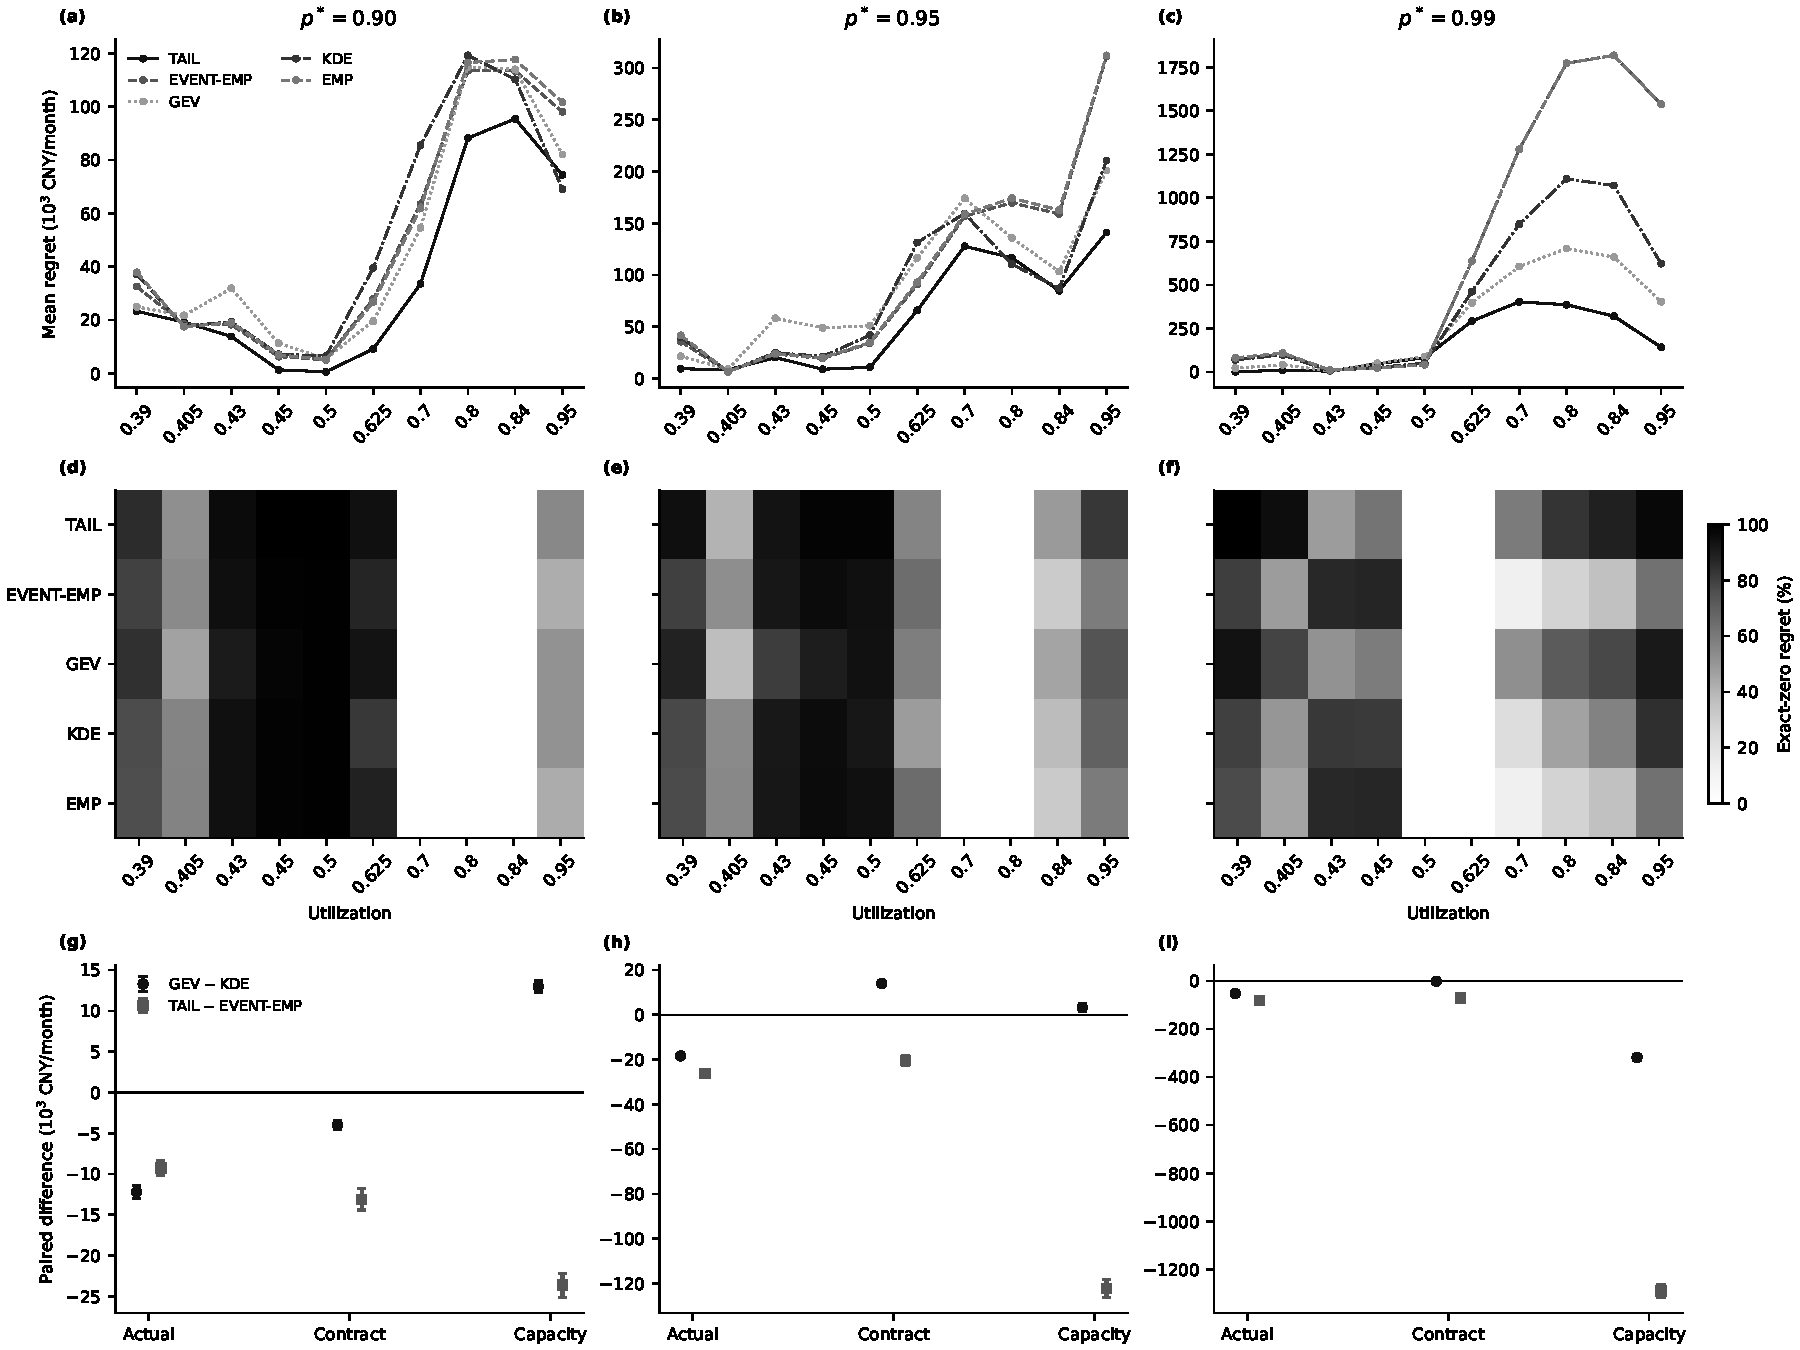
\includegraphics[width=\linewidth]{figures/FigureS1.pdf}
\caption{High-contract-quantile stress using the 10,000 revised primary fitted laws and 1,500,000 tariff decisions. Columns show $p^*=0.90$, $0.95$, and $0.99$. (a--c) Mean full-action regret across the ten utilization cells for each method. (d--f) Exact-zero-regret percentages by method and cell. (g--i) History-paired, equal-cell-weighted regional mean differences for GEV minus KDE and TAIL minus EVENT-EMP, with pointwise 95\% paired $t$ intervals. Negative values favour the first method. The three oracle modes are actual demand, contract demand, and capacity.}
\label{fig:final-figures1}
\end{figure}

\begin{figure}[tbp]
\centering
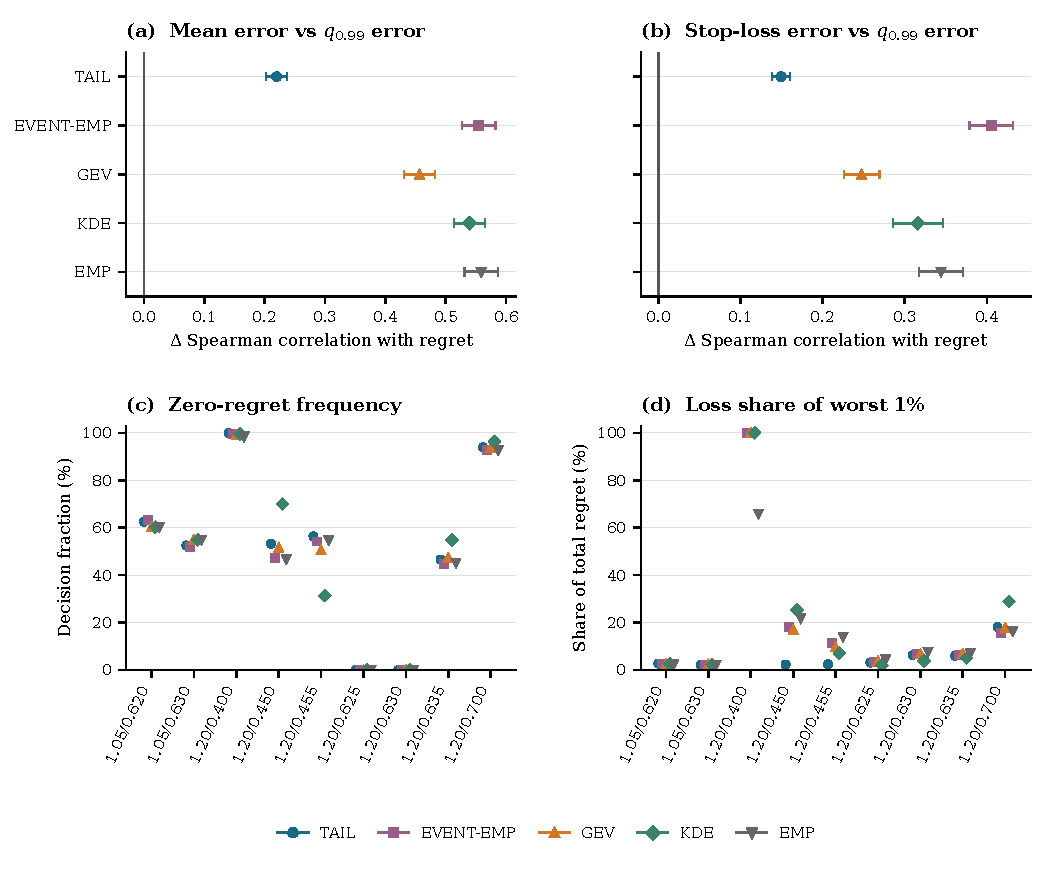
\includegraphics[width=\linewidth]{figures/FigureS2.pdf}
\caption{Functional-error associations and loss concentration. (a,b) Within-method differences between the Spearman correlation of regret with absolute mean or stop-loss relative error and its correlation with absolute $q_{0.99}$ relative error. Error and regret quantities are first averaged over nine cells within each of 10,000 histories. Intervals are the supplied simultaneous max-$|T|$ 95\% intervals for the family of ten correlation differences, based on 2,000 paired-history bootstrap resamples. They are not pointwise intervals. (c) Zero-regret frequency and (d) the share of aggregate regret accounted for by the worst 1\% of decisions within each method--cell sample. The lower panels are descriptive summaries from 10,000 histories per method and cell. Offset, unconnected points distinguish methods at discrete tariff cells; the positions do not form a continuous tariff response.}
\label{fig:final-figures2}
\end{figure}

\begin{figure}[tbp]
\centering
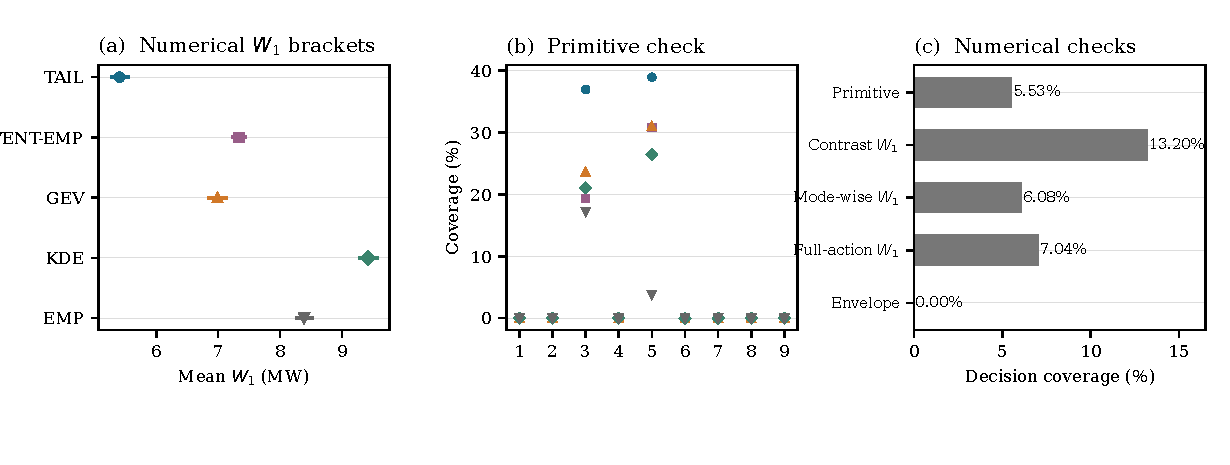
\includegraphics[width=\linewidth]{figures/FigureS3.pdf}
\caption{\textbf{Numerical distribution-to-decision bounds.}
\textbf{(a)} Mean bracket midpoints and adaptive numerical
lower and upper bounds over 10,000 fitted laws per method; the
bounds use adaptive CDF integration and an analytic tail allowance.
\textbf{(b)} Cellwise coverage of the primitive numerical
sufficient-condition check by predictive method.
\textbf{(c)} Overall coverage of the Primitive,
contrast-Wasserstein, mode-wise pairwise-Wasserstein,
full-action regret Wasserstein, and coarse distributional-envelope checks over
450,000 primary decisions. The first four use the same numerical
full-action solver allowance. The contrast-Wasserstein and mode-wise
pairwise-Wasserstein checks differ in whether the common distributional
perturbation is bounded directly for each tariff contrast or after
separate mode-value bounds.
}
\label{fig:final-figures3}
\end{figure}

\begin{figure}[tbp]
\centering
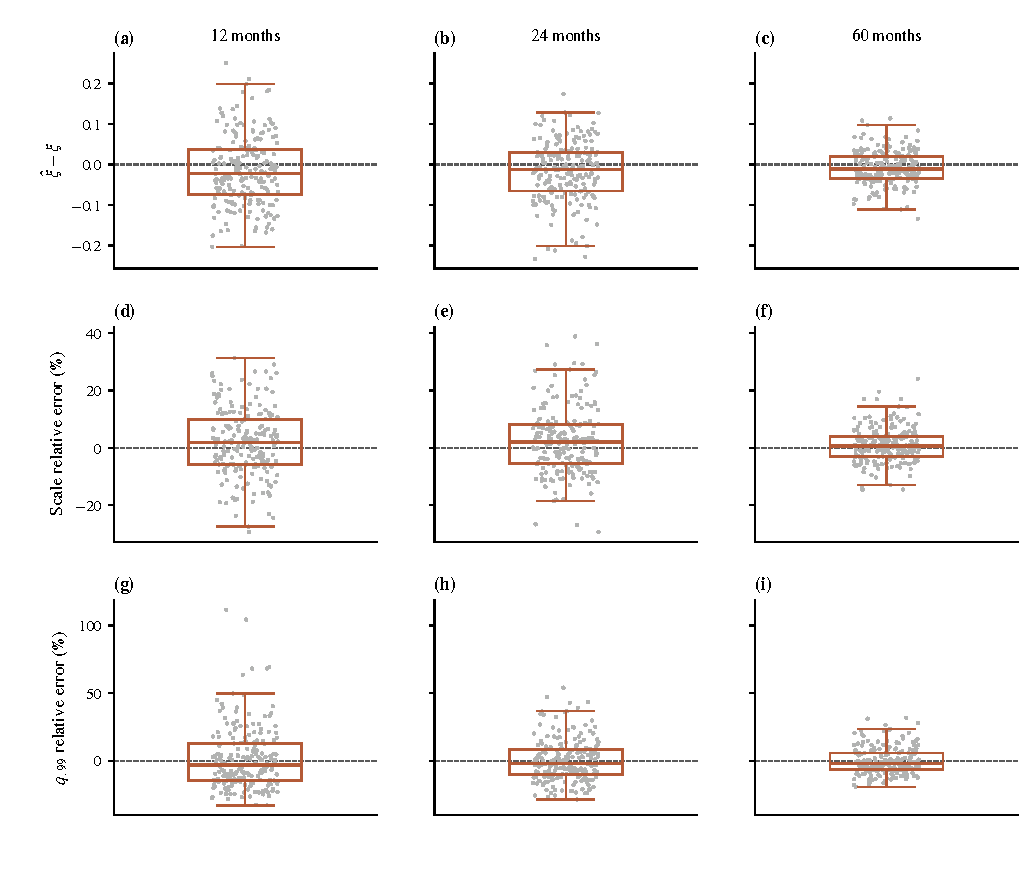
\includegraphics[width=\linewidth]{figures/FigureS4.pdf}
\caption{Parameter-recovery experiment. Columns show training
lengths of 12, 24, and 60 months; rows show GPD shape error, relative
scale error, and relative $q_{0.99}$ error. Each panel displays all
200 histories as grey points, with median, interquartile box, and
1.5-IQR whiskers. These are distribution summaries, not confidence
intervals; the recovery experiment is separate from the primary
analysis.}
\label{fig:final-figures4}
\end{figure}

\begin{figure}[tbp]
\centering
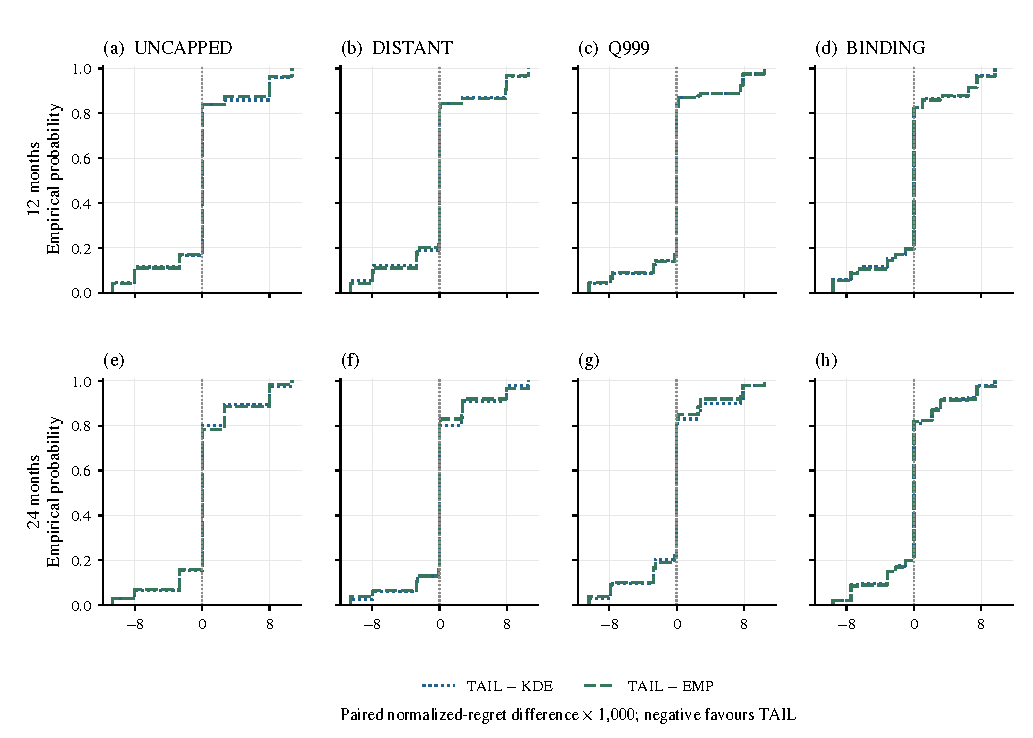
\includegraphics[width=\linewidth]{figures/FigureS5.pdf}
\caption{Physical clipping sensitivity. Columns show the four frozen
clipping regimes and rows show 12 or 24 training months. Each ECDF
contains 200 paired history differences in normalized regret times
1,000; negative values favour TAIL. The full data range is shown, and
the interquartile range is zero in all 16 groups. This descriptive
robustness experiment is separate from the primary analysis.}
\label{fig:final-figures5}
\end{figure}

\begin{figure}[tbp]
\centering
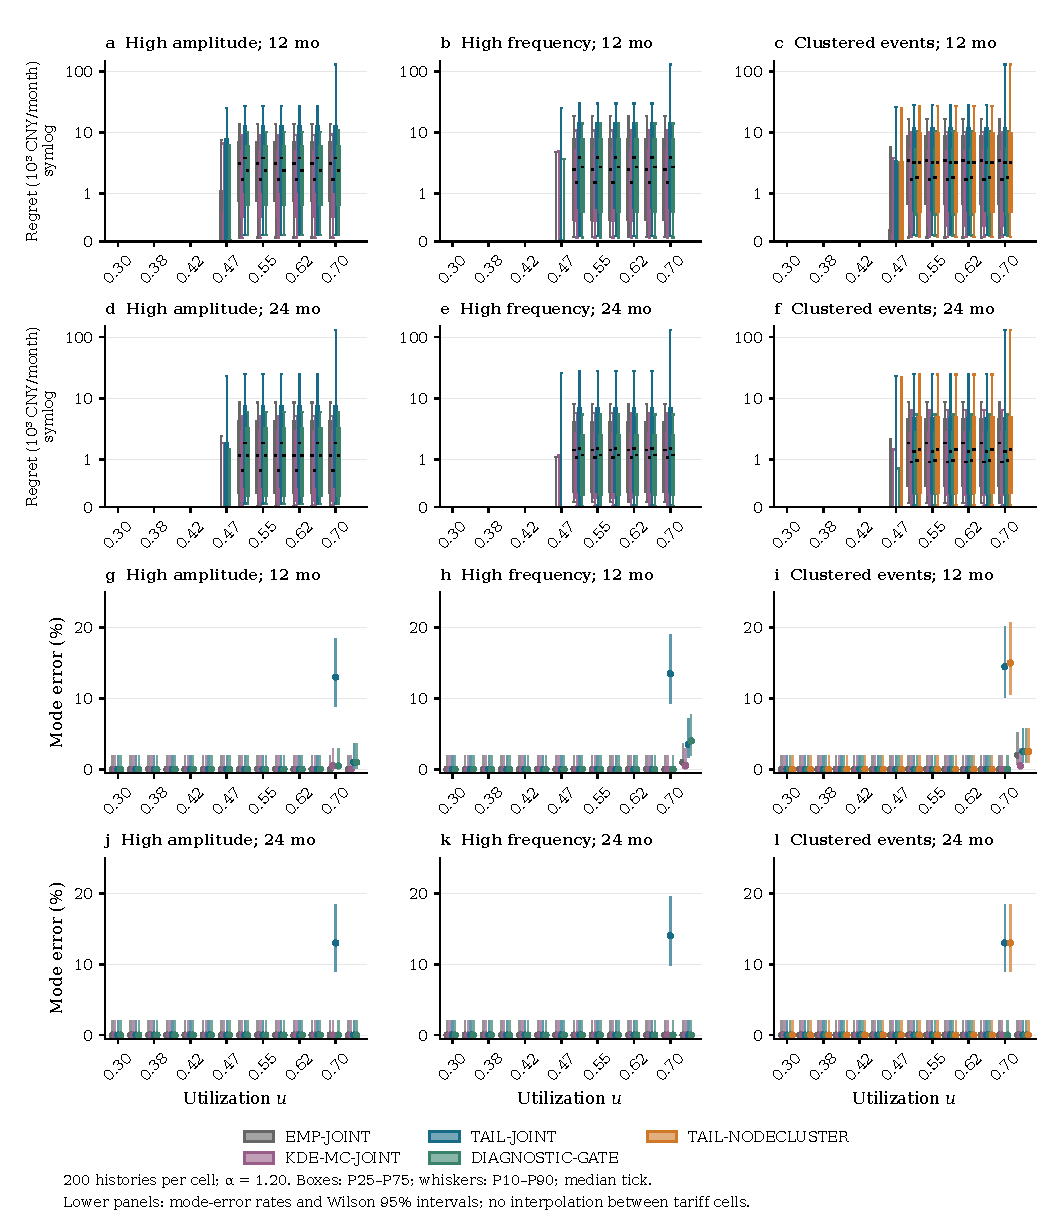
\includegraphics[width=0.94\linewidth]{figures/FigureS6.pdf}
\caption{Physical-pipeline experiments at alpha = 1.20 using 200
paired histories per method, training length, and tariff cell
(72,800 decisions). Columns represent high amplitude, high frequency,
and clustered events. (a--f) Regret distributions at all 14 utilization
cells for training lengths of 12 and 24 months: boxes span P25--P75,
whiskers span P10--P90, and black ticks denote medians. The symlog
ordinate retains zero and is linear below one thousand CNY per month.
Outlying histories beyond the whiskers are not drawn individually;
these are distribution summaries, not confidence intervals. (g--l)
Mode-error proportions and pointwise Wilson 95\% intervals at the
same cells. Points are offset within each cell to separate methods and
are not interpolated between cells. TAIL-NODECLUSTER applies only to
the clustered-event scenario.}
\label{fig:final-figures6}
\end{figure}

\begin{figure}[tbp]
\centering
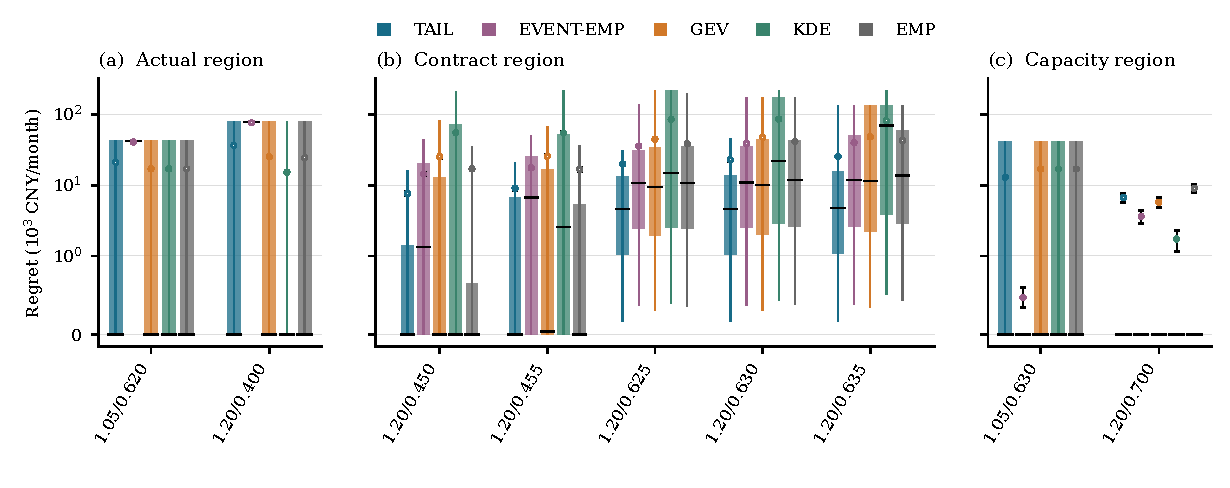
\includegraphics[width=\linewidth]{figures/FigureS7.pdf}
\caption{Cellwise regret distributions under the negative-binomial--Weibull challenge, with 10,000 histories per method and cell. Panels group the two actual, five contract, and two capacity oracle cells; labels give utilization and cells are equally spaced. Filled boxes span P25--P75, black ticks denote medians, whiskers span P10--P90, and open circles denote means. Black intervals at means use the formal pointwise normal 95\% approximation, mean plus or minus 1.96 standard errors. The symlog ordinate is linear below one thousand CNY per month and logarithmic above it. Histories outside the displayed quantile ranges are not drawn individually. Quantile ranges describe history variability and are distinct from uncertainty in the mean.}
\label{fig:final-figures7}
\end{figure}

\begin{figure}[tbp]
\centering
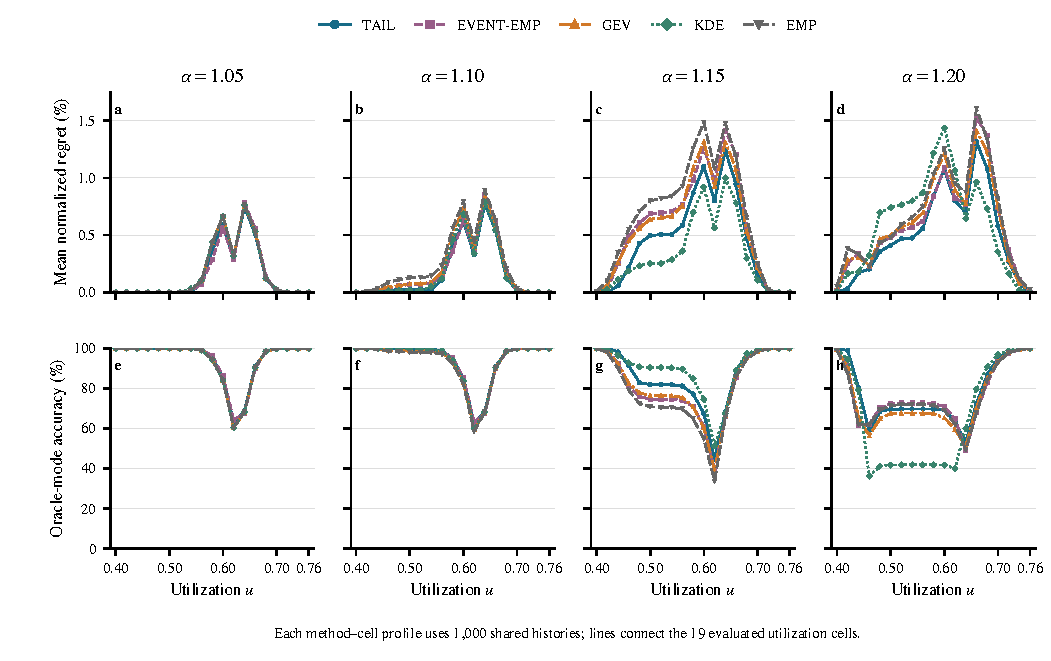
\includegraphics[width=\linewidth]{figures/FigureS8.pdf}
\caption{\textbf{Five-method profiles across the crossed tariff grid.}
Panels (a--d) show mean normalized full-action regret and panels
(e--h) show oracle-mode accuracy for
$\alpha\in\{1.05,1.10,1.15,1.20\}$. Each panel contains the 19
evaluated utilization cells and uses 1,000 shared histories per
method--cell. Lines connect the discrete evaluated cells for visual comparison. No confidence intervals are shown. TAIL and
EVENT--EMP use event-level information, whereas GEV, KDE, and EMP use
monthly maxima.}
\label{fig:crossed-grid-all-methods}
\end{figure}


\clearpage
\subsection*{Supplementary tables}

\begingroup
\fontsize{8.5}{10.5}\selectfont\setlength{\tabcolsep}{3.0pt}\renewcommand{\arraystretch}{1.23}
\begin{table}[tbp]\centering
\caption{Same-information comparisons under high contract quantiles.}\label{tab:si-high-pstar}
\begin{tabular}{@{}llllll@{}}\toprule
$p^*$ & First -- second & Oracle & Cells & Difference & 95\% CI\\\midrule
0.90 & GEV -- KDE & Actual & 1 & -12.19 & [-13.02, -11.36]\\
0.90 & GEV -- KDE & Contract & 8 & -3.97 & [-4.53, -3.41]\\
0.90 & GEV -- KDE & Capacity & 1 & +12.97 & [+12.26, +13.68]\\
0.90 & TAIL -- EVENT-EMP & Actual & 1 & -9.26 & [-10.20, -8.32]\\
0.90 & TAIL -- EVENT-EMP & Contract & 8 & -13.12 & [-14.41, -11.82]\\
0.90 & TAIL -- EVENT-EMP & Capacity & 1 & -23.63 & [-25.10, -22.15]\\
0.95 & GEV -- KDE & Actual & 1 & -18.40 & [-19.46, -17.33]\\
0.95 & GEV -- KDE & Contract & 7 & +13.97 & [+12.78, +15.15]\\
0.95 & GEV -- KDE & Capacity & 2 & +3.28 & [+1.49, +5.07]\\
0.95 & TAIL -- EVENT-EMP & Actual & 1 & -26.19 & [-27.48, -24.91]\\
0.95 & TAIL -- EVENT-EMP & Contract & 7 & -20.36 & [-22.48, -18.24]\\
0.95 & TAIL -- EVENT-EMP & Capacity & 2 & -122.14 & [-126.14, -118.14]\\
0.99 & GEV -- KDE & Actual & 2 & -52.28 & [-54.06, -50.49]\\
0.99 & GEV -- KDE & Contract & 4 & -1.37 & [-3.10, +0.36]\\
0.99 & GEV -- KDE & Capacity & 4 & -318.31 & [-329.72, -306.91]\\
0.99 & TAIL -- EVENT-EMP & Actual & 2 & -81.23 & [-83.31, -79.14]\\
0.99 & TAIL -- EVENT-EMP & Contract & 4 & -71.39 & [-74.16, -68.62]\\
0.99 & TAIL -- EVENT-EMP & Capacity & 4 & -1289.26 & [-1315.73, -1262.79]\\
\bottomrule
\end{tabular}
\par\smallskip\noindent\begin{minipage}{\linewidth}\footnotesize Loss differences are in $10^3$ CNY/month. Each comparison uses the same 10,000 fitted primary histories and equal weights over the indicated region cells; intervals are pointwise paired $t$ intervals. Alpha is 2.20.\end{minipage}
\end{table}
\endgroup

\FloatBarrier

\begingroup
\fontsize{8.5}{10.5}\selectfont\setlength{\tabcolsep}{3.0pt}\renewcommand{\arraystretch}{1.23}
\begin{table}[tbp]\centering
\caption{Within-contract regret by mode-stability condition.}\label{tab:si-stability-condition}
\begin{tabular}{@{}lllllll@{}}\toprule
Condition & Method & Satisfied & Decisions & Histories & Mean & 95\% CI\\\midrule
$d_{MV}$ & TAIL & Yes & 458 & 395 & 0.36 & [0.31, 0.42]\\
$d_{MV}$ & TAIL & No & 16,541 & 6,605 & 8.09 & [7.74, 8.43]\\
$d_{MV}$ & EVENT-EMP & Yes & 284 & 254 & 7.14 & [5.86, 8.43]\\
$d_{MV}$ & EVENT-EMP & No & 17,581 & 6,948 & 11.73 & [11.26, 12.20]\\
$d_{MV}$ & GEV & Yes & 228 & 208 & 4.23 & [3.50, 4.95]\\
$d_{MV}$ & GEV & No & 16,308 & 6,658 & 13.11 & [12.56, 13.65]\\
$d_{MV}$ & KDE & Yes & 144 & 131 & 12.19 & [10.42, 13.96]\\
$d_{MV}$ & KDE & No & 10,684 & 4,273 & 9.75 & [9.22, 10.28]\\
$d_{MV}$ & EMP & Yes & 221 & 201 & 8.80 & [7.11, 10.48]\\
$d_{MV}$ & EMP & No & 17,285 & 6,995 & 17.86 & [17.16, 18.56]\\
Pairwise-gap & TAIL & Yes & 1,026 & 666 & 0.59 & [0.52, 0.65]\\
Pairwise-gap & TAIL & No & 15,973 & 6,371 & 8.35 & [7.99, 8.70]\\
Pairwise-gap & EVENT-EMP & Yes & 714 & 465 & 7.61 & [6.64, 8.58]\\
Pairwise-gap & EVENT-EMP & No & 17,151 & 6,813 & 11.73 & [11.25, 12.21]\\
Pairwise-gap & GEV & Yes & 598 & 394 & 4.42 & [3.81, 5.02]\\
Pairwise-gap & GEV & No & 15,938 & 6,526 & 13.24 & [12.68, 13.79]\\
Pairwise-gap & KDE & Yes & 408 & 262 & 11.93 & [10.71, 13.14]\\
Pairwise-gap & KDE & No & 10,420 & 4,220 & 9.58 & [9.04, 10.11]\\
Pairwise-gap & EMP & Yes & 580 & 379 & 10.04 & [8.47, 11.61]\\
Pairwise-gap & EMP & No & 16,926 & 6,891 & 17.84 & [17.13, 18.55]\\
\bottomrule
\end{tabular}
\par\smallskip\noindent\begin{minipage}{\linewidth}\footnotesize The subset contains decisions for which both oracle and fitted-law selected modes are contract. The mean is the equally weighted mean of eligible history means, with a pointwise $t$ interval using the displayed number of histories. Loss units are $10^3$ CNY/month. Different subsets overlap across methods and condition strata; their counts must not be added to obtain the number of independent histories.\end{minipage}
\end{table}
\endgroup

\FloatBarrier

\begingroup
\fontsize{7.5}{9.5}\selectfont\setlength{\tabcolsep}{2.5pt}\renewcommand{\arraystretch}{1.23}
\begin{table}[tbp]\centering
\caption{Physical-mechanism stress tests at alpha 1.20.}\label{tab:si-s6-updated}
\resizebox{\linewidth}{!}{\begin{tabular}{@{}llllllll@{}}\toprule
Scenario & Months & Method & Regret & MCSE & Mode & Within & Error (\%)\\\midrule
High amplitude & 12 & GATE & 2.114 & 0.236 & 0.110 & 2.005 & 0.107\\
High amplitude & 12 & EMP-JOINT & 2.512 & 0.248 & 0.000 & 2.512 & 0.000\\
High amplitude & 12 & KDE-MC-JOINT & 1.783 & 0.200 & 0.046 & 1.737 & 0.036\\
High amplitude & 12 & TAIL-JOINT & 5.740 & 0.653 & 1.267 & 4.473 & 1.000\\
High amplitude & 24 & GATE & 0.997 & 0.090 & 0.000 & 0.997 & 0.000\\
High amplitude & 24 & EMP-JOINT & 1.283 & 0.117 & 0.000 & 1.283 & 0.000\\
High amplitude & 24 & KDE-MC-JOINT & 0.842 & 0.079 & 0.000 & 0.842 & 0.000\\
High amplitude & 24 & TAIL-JOINT & 4.451 & 0.534 & 1.204 & 3.247 & 0.929\\
High frequency & 12 & GATE & 2.589 & 0.277 & 0.253 & 2.336 & 0.286\\
High frequency & 12 & EMP-JOINT & 2.731 & 0.274 & 0.063 & 2.668 & 0.071\\
High frequency & 12 & KDE-MC-JOINT & 1.784 & 0.185 & 0.032 & 1.752 & 0.036\\
High frequency & 12 & TAIL-JOINT & 5.937 & 0.621 & 1.472 & 4.464 & 1.214\\
High frequency & 24 & GATE & 0.947 & 0.090 & 0.000 & 0.947 & 0.000\\
High frequency & 24 & EMP-JOINT & 1.286 & 0.116 & 0.000 & 1.286 & 0.000\\
High frequency & 24 & KDE-MC-JOINT & 0.948 & 0.095 & 0.000 & 0.948 & 0.000\\
High frequency & 24 & TAIL-JOINT & 4.311 & 0.544 & 1.297 & 3.014 & 1.000\\
Clustered events & 12 & GATE & 2.151 & 0.264 & 0.158 & 1.993 & 0.179\\
Clustered events & 12 & EMP-JOINT & 3.135 & 0.315 & 0.127 & 3.009 & 0.143\\
Clustered events & 12 & KDE-MC-JOINT & 1.855 & 0.217 & 0.032 & 1.823 & 0.036\\
Clustered events & 12 & TAIL-JOINT & 5.303 & 0.582 & 1.502 & 3.801 & 1.214\\
Clustered events & 12 & TAIL-NODECLUSTER & 5.380 & 0.595 & 1.548 & 3.832 & 1.250\\
Clustered events & 24 & GATE & 0.936 & 0.093 & 0.000 & 0.936 & 0.000\\
Clustered events & 24 & EMP-JOINT & 1.572 & 0.145 & 0.000 & 1.572 & 0.000\\
Clustered events & 24 & KDE-MC-JOINT & 1.020 & 0.105 & 0.000 & 1.020 & 0.000\\
Clustered events & 24 & TAIL-JOINT & 3.782 & 0.513 & 1.205 & 2.577 & 0.929\\
Clustered events & 24 & TAIL-NODECLUSTER & 3.768 & 0.510 & 1.205 & 2.563 & 0.929\\
\bottomrule
\end{tabular}}
\par\smallskip\noindent\begin{minipage}{\linewidth}\footnotesize Each scenario-by-training-length summary uses 200 independent sampled histories, each evaluated at 14 equally weighted tariff cells (2,800 decision rows). GATE denotes DIAGNOSTIC-GATE. Losses are in $10^3$ CNY/month. MCSEs are calculated across the 200 histories after averaging cells within history and are conditional on the fixed 5,000-month training library and 20,000-month test pool. The oracle is the fixed 20,000-month test-pool benchmark.\end{minipage}
\end{table}
\endgroup

\FloatBarrier

\begingroup
\fontsize{8.5}{10.5}\selectfont\setlength{\tabcolsep}{3pt}
\begin{longtable}{@{}llllll@{}}
\caption{Cell-specific NB--Weibull challenge results.}\label{tab:final-si-4}\\
\toprule
Region & Alpha / $u$ & Method & Mean regret & 95\% CI & Accuracy (\%)\\\midrule\endfirsthead
Region & Alpha / $u$ & Method & Mean regret & 95\% CI & Accuracy (\%)\\\midrule\endhead
actual & 1.05 / 0.620 & EMP & 17.05 & [16.64, 17.45] & 59.7\\
capacity & 1.05 / 0.630 & EMP & 16.96 & [16.56, 17.36] & 59.3\\
actual & 1.20 / 0.400 & EMP & 24.55 & [23.83, 25.27] & 68.9\\
contract & 1.20 / 0.450 & EMP & 17.01 & [16.01, 18.01] & 93.9\\
contract & 1.20 / 0.455 & EMP & 16.82 & [15.86, 17.79] & 94.8\\
contract & 1.20 / 0.625 & EMP & 38.49 & [37.23, 39.76] & 90.1\\
contract & 1.20 / 0.630 & EMP & 41.54 & [40.31, 42.77] & 86.2\\
contract & 1.20 / 0.635 & EMP & 42.65 & [41.53, 43.77] & 81.3\\
capacity & 1.20 / 0.700 & EMP & 9.05 & [7.83, 10.27] & 97.9\\
actual & 1.05 / 0.620 & EVENT-EMP & 40.83 & [40.64, 41.02] & 3.7\\
capacity & 1.05 / 0.630 & EVENT-EMP & 0.47 & [0.34, 0.60] & 99.0\\
actual & 1.20 / 0.400 & EVENT-EMP & 76.46 & [76.18, 76.73] & 3.2\\
contract & 1.20 / 0.450 & EVENT-EMP & 14.39 & [13.91, 14.87] & 100.0\\
contract & 1.20 / 0.455 & EVENT-EMP & 17.60 & [17.09, 18.10] & 100.0\\
contract & 1.20 / 0.625 & EVENT-EMP & 35.85 & [34.61, 37.08] & 90.0\\
contract & 1.20 / 0.630 & EVENT-EMP & 39.05 & [37.86, 40.24] & 84.5\\
contract & 1.20 / 0.635 & EVENT-EMP & 40.05 & [39.01, 41.09] & 77.4\\
capacity & 1.20 / 0.700 & EVENT-EMP & 3.62 & [2.90, 4.34] & 99.0\\
actual & 1.05 / 0.620 & GEV & 17.11 & [16.70, 17.52] & 59.6\\
capacity & 1.05 / 0.630 & GEV & 16.89 & [16.49, 17.29] & 59.4\\
actual & 1.20 / 0.400 & GEV & 25.29 & [24.56, 26.01] & 68.0\\
contract & 1.20 / 0.450 & GEV & 25.41 & [24.24, 26.59] & 91.2\\
contract & 1.20 / 0.455 & GEV & 25.59 & [24.45, 26.74] & 92.2\\
contract & 1.20 / 0.625 & GEV & 44.86 & [43.38, 46.34] & 84.6\\
contract & 1.20 / 0.630 & GEV & 47.69 & [46.29, 49.10] & 79.8\\
contract & 1.20 / 0.635 & GEV & 48.33 & [47.07, 49.58] & 73.5\\
capacity & 1.20 / 0.700 & GEV & 5.75 & [4.79, 6.71] & 98.6\\
actual & 1.05 / 0.620 & KDE & 17.05 & [16.64, 17.45] & 59.7\\
capacity & 1.05 / 0.630 & KDE & 16.96 & [16.56, 17.36] & 59.3\\
actual & 1.20 / 0.400 & KDE & 15.23 & [14.62, 15.84] & 80.7\\
contract & 1.20 / 0.450 & KDE & 55.44 & [53.71, 57.17] & 75.9\\
contract & 1.20 / 0.455 & KDE & 54.95 & [53.22, 56.67] & 77.5\\
contract & 1.20 / 0.625 & KDE & 85.43 & [83.46, 87.40] & 63.7\\
contract & 1.20 / 0.630 & KDE & 86.07 & [84.29, 87.84] & 57.7\\
contract & 1.20 / 0.635 & KDE & 81.62 & [80.10, 83.14] & 50.8\\
capacity & 1.20 / 0.700 & KDE & 1.73 & [1.16, 2.30] & 99.6\\
actual & 1.05 / 0.620 & TAIL & 21.09 & [20.68, 21.51] & 50.1\\
capacity & 1.05 / 0.630 & TAIL & 12.98 & [12.61, 13.36] & 68.8\\
actual & 1.20 / 0.400 & TAIL & 36.50 & [35.73, 37.27] & 53.8\\
contract & 1.20 / 0.450 & TAIL & 7.63 & [7.05, 8.22] & 98.1\\
contract & 1.20 / 0.455 & TAIL & 9.03 & [8.46, 9.60] & 98.4\\
contract & 1.20 / 0.625 & TAIL & 19.94 & [18.98, 20.91] & 94.4\\
contract & 1.20 / 0.630 & TAIL & 23.02 & [22.03, 24.01] & 91.1\\
contract & 1.20 / 0.635 & TAIL & 25.46 & [24.52, 26.40] & 86.3\\
capacity & 1.20 / 0.700 & TAIL & 6.71 & [5.69, 7.73] & 98.3\\
\bottomrule
\end{longtable}
\endgroup

\FloatBarrier

\begingroup
\fontsize{8.5}{10.5}\selectfont\setlength{\tabcolsep}{3pt}
\begin{longtable}{@{}llll@{}}
\caption{Complete regional paired NB--Weibull contrasts.}\label{tab:final-si-5}\\
\toprule
Region & First -- second & Mean difference & 95\% CI\\\midrule\endfirsthead
Region & First -- second & Mean difference & 95\% CI\\\midrule\endhead
actual & TAIL -- EVENT-EMP & -29.85 & [-30.42, -29.28]\\
actual & TAIL -- GEV & +7.60 & [+7.11, +8.08]\\
actual & TAIL -- KDE & +12.66 & [+12.17, +13.14]\\
actual & TAIL -- EMP & +8.00 & [+7.51, +8.48]\\
actual & EVENT-EMP -- GEV & +37.45 & [+36.91, +37.99]\\
actual & EVENT-EMP -- KDE & +42.51 & [+42.03, +42.98]\\
actual & EVENT-EMP -- EMP & +37.85 & [+37.31, +38.38]\\
actual & GEV -- KDE & +5.06 & [+4.80, +5.32]\\
actual & GEV -- EMP & +0.40 & [+0.25, +0.55]\\
actual & KDE -- EMP & -4.66 & [-4.91, -4.41]\\
contract & TAIL -- EVENT-EMP & -12.37 & [-13.06, -11.69]\\
contract & TAIL -- GEV & -21.36 & [-22.36, -20.36]\\
contract & TAIL -- KDE & -55.69 & [-57.16, -54.21]\\
contract & TAIL -- EMP & -14.29 & [-15.16, -13.41]\\
contract & EVENT-EMP -- GEV & -8.99 & [-9.99, -7.99]\\
contract & EVENT-EMP -- KDE & -43.31 & [-44.77, -41.86]\\
contract & EVENT-EMP -- EMP & -1.91 & [-2.83, -1.00]\\
contract & GEV -- KDE & -34.32 & [-35.51, -33.14]\\
contract & GEV -- EMP & +7.08 & [+6.46, +7.69]\\
contract & KDE -- EMP & +41.40 & [+40.08, +42.71]\\
capacity & TAIL -- EVENT-EMP & +7.81 & [+7.35, +8.26]\\
capacity & TAIL -- GEV & -1.47 & [-1.93, -1.02]\\
capacity & TAIL -- KDE & +0.50 & [-0.01, +1.02]\\
capacity & TAIL -- EMP & -3.16 & [-3.67, -2.65]\\
capacity & EVENT-EMP -- GEV & -9.28 & [-9.70, -8.86]\\
capacity & EVENT-EMP -- KDE & -7.30 & [-7.74, -6.87]\\
capacity & EVENT-EMP -- EMP & -10.96 & [-11.49, -10.44]\\
capacity & GEV -- KDE & +1.98 & [+1.58, +2.37]\\
capacity & GEV -- EMP & -1.68 & [-2.04, -1.33]\\
capacity & KDE -- EMP & -3.66 & [-4.20, -3.12]\\
\bottomrule
\end{longtable}
\endgroup

\FloatBarrier

\begingroup
\fontsize{8.5}{10.5}\selectfont\setlength{\tabcolsep}{3pt}
\begin{longtable}{@{}llll@{}}
\caption{Numerical Wasserstein brackets.}\label{tab:final-si-6}\\
\toprule
Method & Mean W1 (MW) & Mean lower (MW) & Mean upper (MW)\\\midrule\endfirsthead
Method & Mean W1 (MW) & Mean lower (MW) & Mean upper (MW)\\\midrule\endhead
EMP & 8.390 & 8.268 & 8.513\\
EVENT-EMP & 7.339 & 7.240 & 7.439\\
GEV & 6.988 & 6.857 & 7.120\\
KDE & 9.425 & 9.290 & 9.559\\
TAIL & 5.408 & 5.278 & 5.538\\
\bottomrule
\end{longtable}
\noindent\footnotesize Point values are midpoints of the combined numerical $W_1$ brackets, formed by intersecting adaptive CDF and archived monotone-CDF brackets. Columns average 10,000 fitted laws per method. Bounds include an analytic tail allowance.
\endgroup

\FloatBarrier

\begingroup
\fontsize{8.5}{10.5}\selectfont\setlength{\tabcolsep}{3pt}
\begin{longtable}{@{}llll@{}}
\caption{Functional-error correlation contrasts.}\label{tab:final-si-7}\\
\toprule
Method & Contrast & Estimate & Simultaneous 95\% CI\\\midrule\endfirsthead
Method & Contrast & Estimate & Simultaneous 95\% CI\\\midrule\endhead
TAIL & Mean -- q99 & +0.193 & [+0.176, +0.210]\\
TAIL & Stop-loss -- q99 & +0.132 & [+0.121, +0.143]\\
EVENT-EMP & Mean -- q99 & +0.555 & [+0.527, +0.583]\\
EVENT-EMP & Stop-loss -- q99 & +0.405 & [+0.379, +0.432]\\
GEV & Mean -- q99 & +0.457 & [+0.430, +0.483]\\
GEV & Stop-loss -- q99 & +0.247 & [+0.226, +0.269]\\
KDE & Mean -- q99 & +0.539 & [+0.514, +0.565]\\
KDE & Stop-loss -- q99 & +0.316 & [+0.285, +0.347]\\
EMP & Mean -- q99 & +0.559 & [+0.531, +0.587]\\
EMP & Stop-loss -- q99 & +0.344 & [+0.317, +0.371]\\
\bottomrule
\end{longtable}
\noindent\footnotesize The supplied max-$|T|$ intervals cover the family of ten within-method correlation differences. Resampling unit: history; 2,000 paired bootstrap resamples. Nine cells are averaged within each of 10,000 histories.
\endgroup

\FloatBarrier

\begingroup
\fontsize{8.5}{10.5}\selectfont\setlength{\tabcolsep}{3pt}
\begin{longtable}{@{}lll@{}}
\caption{External fit-status counts, natural-tail variant.}\label{tab:final-si-8}\\
\toprule
Method & Formal fit status & Factory-origin fits\\\midrule\endfirsthead
Method & Formal fit status & Factory-origin fits\\\midrule\endhead
K-BLOCK & PASS & 32\\
K-EMP & PASS & 32\\
K-GEV & FALLBACK\_EMPIRICAL & 24\\
K-GEV & PASS & 8\\
K-GTAIL & FALLBACK\_EMPIRICAL & 4\\
K-GTAIL & FALLBACK\_EXPONENTIAL & 13\\
K-GTAIL & PASS & 15\\
K-KDE & PASS & 32\\
K-POINT & PASS & 32\\
K-UGPD & PASS & 32\\
\bottomrule
\end{longtable}
\noindent\footnotesize Eight factories and four rolling origins yield 32 fits per method. Labels are the formal stored status labels; fallback fits remain part of the evaluated pipeline.
\endgroup

\FloatBarrier

\begingroup
\fontsize{8.5}{10.5}\selectfont\setlength{\tabcolsep}{3pt}
\begin{longtable}{@{}llll@{}}
\caption{External predictive-score paired contrasts of K-GTAIL with six alternative procedures.}\label{tab:final-si-9}\\
\toprule
Score & Baseline & K-GTAIL -- baseline & 95\% CI\\\midrule\endfirsthead
Score & Baseline & K-GTAIL -- baseline & 95\% CI\\\midrule\endhead
CRPS & K-BLOCK & +5.627 & [-9.534, +20.789]\\
CRPS & K-EMP & +3.005 & [-13.858, +19.869]\\
CRPS & K-GEV & +3.002 & [-14.318, +20.323]\\
CRPS & K-KDE & +4.654 & [-11.430, +20.737]\\
CRPS & K-POINT & -3.638 & [-23.912, +16.635]\\
CRPS & K-UGPD & +5.433 & [-10.773, +21.640]\\
Weighted CRPS (0.90) & K-BLOCK & -0.510 & [-1.895, +0.876]\\
Weighted CRPS (0.90) & K-EMP & -0.510 & [-1.895, +0.876]\\
Weighted CRPS (0.90) & K-GEV & -0.613 & [-2.177, +0.950]\\
Weighted CRPS (0.90) & K-KDE & -0.087 & [-0.938, +0.765]\\
Weighted CRPS (0.90) & K-POINT & -2.612 & [-6.377, +1.153]\\
Weighted CRPS (0.90) & K-UGPD & -0.239 & [-1.646, +1.168]\\
Pinball ($q_{0.95}$) & K-BLOCK & -2.594 & [-10.152, +4.964]\\
Pinball ($q_{0.95}$) & K-EMP & -2.594 & [-10.152, +4.964]\\
Pinball ($q_{0.95}$) & K-GEV & -3.268 & [-11.774, +5.239]\\
Pinball ($q_{0.95}$) & K-KDE & -0.548 & [-5.256, +4.161]\\
Pinball ($q_{0.95}$) & K-POINT & -13.777 & [-33.874, +6.319]\\
Pinball ($q_{0.95}$) & K-UGPD & -1.447 & [-9.258, +6.363]\\
Pinball ($q_{0.99}$) & K-BLOCK & -4.071 & [-11.427, +3.285]\\
Pinball ($q_{0.99}$) & K-EMP & -4.071 & [-11.427, +3.285]\\
Pinball ($q_{0.99}$) & K-GEV & -4.481 & [-12.648, +3.687]\\
Pinball ($q_{0.99}$) & K-KDE & -0.050 & [-2.356, +2.256]\\
Pinball ($q_{0.99}$) & K-POINT & -17.134 & [-37.650, +3.382]\\
Pinball ($q_{0.99}$) & K-UGPD & -0.993 & [-5.021, +3.034]\\
\bottomrule
\end{longtable}
\noindent\footnotesize Scores and intervals are multiplied by $10^3$. Each factory averages four origins; pointwise paired $t$ intervals use eight factory differences and seven degrees of freedom. Score-specific comparisons are descriptive.
\endgroup

\FloatBarrier

% Requires booktabs, array, longtable.
{\small
\begin{longtable}{>{\raggedright\arraybackslash}p{48pt}>{\raggedright\arraybackslash}p{64pt}>{\raggedright\arraybackslash}p{76pt}>{\raggedright\arraybackslash}p{132pt}}
\caption{Conditional parameter-interval coverage}\label{tab:table_s10}\\
\toprule
\textbf{Months} & \textbf{Parameter} & \textbf{Covered /\allowbreak{} histories} & \textbf{Coverage (\%) [95\% MC CI]} \\
\midrule\endfirsthead
\toprule
\textbf{Months} & \textbf{Parameter} & \textbf{Covered /\allowbreak{} histories} & \textbf{Coverage (\%) [95\% MC CI]} \\
\midrule\endhead
\bottomrule\endfoot
12 & xi & 182 /\allowbreak{} 200 & 91.00 [86.15, 94.58] \\
12 & sigma & 190 /\allowbreak{} 200 & 95.00 [91.00, 97.58] \\
24 & xi & 185 /\allowbreak{} 200 & 92.50 [87.93, 95.74] \\
24 & sigma & 182 /\allowbreak{} 200 & 91.00 [86.15, 94.58] \\
60 & xi & 190 /\allowbreak{} 200 & 95.00 [91.00, 97.58] \\
60 & sigma & 191 /\allowbreak{} 200 & 95.50 [91.63, 97.92] \\
\end{longtable}
\noindent{\footnotesize Separate inherited recovery experiment, 200 histories per setting; not the primary experiment. Coverage conditions on the selected threshold. Clopper--Pearson intervals describe Monte Carlo uncertainty in coverage.\par}
}

\FloatBarrier


\begingroup
\fontsize{8.5}{10.5}\selectfont\setlength{\tabcolsep}{3.0pt}\renewcommand{\arraystretch}{1.23}
\begin{table}[tbp]\centering
\caption{Complete history-paired regret contrasts in the primary experiment.}\label{tab:final-si-11}
\begin{tabular}{@{}llll@{}}\toprule
First -- second & Actual & Contract & Capacity\\\midrule
TAIL -- EVENT-EMP & \shortstack{-0.48\\{}[-0.65, -0.32]} & \shortstack{-1.16\\{}[-1.40, -0.92]} & \shortstack{-3.64\\{}[-4.25, -3.04]}\\
GEV -- KDE & \shortstack{+0.82\\{}[+0.68, +0.97]} & \shortstack{-3.89\\{}[-4.14, -3.63]} & \shortstack{+5.47\\{}[+4.87, +6.07]}\\
KDE -- EMP & \shortstack{-1.66\\{}[-1.88, -1.43]} & \shortstack{+1.73\\{}[+1.40, +2.06]} & \shortstack{-8.71\\{}[-9.41, -8.00]}\\
TAIL -- KDE & \shortstack{-0.53\\{}[-0.73, -0.34]} & \shortstack{-6.86\\{}[-7.17, -6.55]} & \shortstack{+3.16\\{}[+2.52, +3.80]}\\
TAIL -- GEV & \shortstack{-1.36\\{}[-1.60, -1.11]} & \shortstack{-2.97\\{}[-3.24, -2.70]} & \shortstack{-2.31\\{}[-2.94, -1.69]}\\
TAIL -- EMP & \shortstack{-2.19\\{}[-2.49, -1.89]} & \shortstack{-5.13\\{}[-5.46, -4.79]} & \shortstack{-5.55\\{}[-6.23, -4.86]}\\
GEV -- EMP & \shortstack{-0.84\\{}[-1.01, -0.66]} & \shortstack{-2.16\\{}[-2.37, -1.95]} & \shortstack{-3.23\\{}[-3.62, -2.85]}\\
EVENT-EMP -- GEV & \shortstack{-0.88\\{}[-1.12, -0.63]} & \shortstack{-1.81\\{}[-2.05, -1.57]} & \shortstack{+1.33\\{}[+0.77, +1.89]}\\
EVENT-EMP -- KDE & \shortstack{-0.05\\{}[-0.26, +0.15]} & \shortstack{-5.70\\{}[-5.99, -5.40]} & \shortstack{+6.80\\{}[+6.10, +7.50]}\\
EVENT-EMP -- EMP & \shortstack{-1.71\\{}[-1.99, -1.43]} & \shortstack{-3.97\\{}[-4.25, -3.68]} & \shortstack{-1.90\\{}[-2.46, -1.35]}\\
\bottomrule
\end{tabular}
\par\smallskip\noindent\begin{minipage}{\linewidth}\footnotesize First method minus second, in $10^3$ CNY/month; negative values favour the first method. Brackets are pointwise paired $t$ 95\% intervals from 10,000 equally weighted regional history means (9,999 degrees of freedom). The first two comparisons share event histories and monthly maxima, respectively; the remaining comparisons provide descriptive context. Intervals are not simultaneous and are not interpreted as family-wise evidence.\end{minipage}
\end{table}
\endgroup

\FloatBarrier

\begingroup
\small
\setlength{\tabcolsep}{2.5pt}
\renewcommand{\arraystretch}{1.12}
\begin{table}[tbp]
\centering
\caption{Primary tariff geometry and analytic demand-scale stability radii.}
\label{tab:analytic-demand-radii}
\resizebox{\linewidth}{!}{%
\begin{tabular}{@{}rrlrrrrrr@{}}
\toprule
$\alpha$ & Utilization & Oracle mode & $V_F^*$ & $\gamma_F$ & Relative gap & $\rho_F^{\mathrm{contrast}}$ & $\rho_F^{\mathrm{pair}}$ & $\rho_F$ \\
& & & \shortstack{($10^3$ CNY/month)} & \shortstack{($10^3$ CNY/month)} & (\%) & (kW) & (kW) & (kW) \\
\midrule
1.05 & 0.620 & Actual & 5,336.473 & 43.036 & 0.806 & 1,195.45 & 1,195.45 & 298.86 \\
1.05 & 0.630 & Capacity & 5,294.120 & 42.353 & 0.800 & 1,176.47 & 1,176.47 & 294.12 \\
1.20 & 0.400 & Actual & 5,336.473 & 318.649 & 5.971 & 8,851.37 & 2,950.46 & 2,212.84 \\
1.20 & 0.450 & Actual & 5,336.473 & 4.962 & 0.093 & 137.84 & 45.95 & 34.46 \\
1.20 & 0.455 & Contract & 5,324.612 & 11.861 & 0.223 & 329.48 & 109.83 & 82.37 \\
1.20 & 0.625 & Contract & 5,276.065 & 60.408 & 1.145 & 839.00 & 559.34 & 419.50 \\
1.20 & 0.630 & Contract & 5,276.065 & 18.055 & 0.342 & 250.77 & 250.77 & 125.38 \\
1.20 & 0.635 & Capacity & 5,252.434 & 23.631 & 0.450 & 328.20 & 328.20 & 164.10 \\
1.20 & 0.700 & Capacity & 4,764.708 & 511.357 & 10.732 & 7,102.18 & 7,102.18 & 3,551.09 \\
\bottomrule
\end{tabular}}
\par\smallskip
\begin{minipage}{\linewidth}\footnotesize $V_F^*$ and $\gamma_F$ are in thousand CNY/month; relative gap is $100\gamma_F/V_F^*$. The direct contrast radius is $\rho_F^{\mathrm{contrast}}=\min_{m\neq m_F^*}\gamma_{F,m}/K_{m,m_F^*}$; the mode-wise pairwise radius is $\rho_F^{\mathrm{pair}}=\min_{m\neq m_F^*}\gamma_{F,m}/(L_m+L_{m_F^*})$; and the uniform radius is $\rho_F=\gamma_F/(2L)$ with $L=r_d\max\{1,\kappa\}$. All are oracle-dependent analytic quantities in kW and contain no numerical-integration or solver allowance. For the primary coefficients, $\kappa=2$, so $K_{\mathrm{act},\mathrm{con}}=36\,\mathrm{CNY/(kW\cdot month)}$ compared with $L_{\mathrm{act}}+L_{\mathrm{con}}=108\,\mathrm{CNY/(kW\cdot month)}$. Across these cells, $\rho_F^{\mathrm{contrast}}\geq\rho_F^{\mathrm{pair}}\geq\rho_F$.\end{minipage}
\end{table}
\endgroup

\FloatBarrier

\begingroup
\small
\setlength{\tabcolsep}{5pt}
\renewcommand{\arraystretch}{1.15}
\begin{table}[tbp]
\centering
\caption{Numerical sufficient-condition implementation checks.}
\label{tab:numerical-sufficient-condition-audit}
\resizebox{\linewidth}{!}{\begin{tabular}{@{}lrrr@{}}
\toprule
Condition & Passing rows & Coverage (\%) & Observed mode-selection violations \\
\midrule
Primitive numerical check & 24,894 & 5.532000 & 0 \\
Contrast-Wasserstein numerical check & 59,410 & 13.202222 & 0 \\
Mode-wise pairwise-Wasserstein numerical check & 27,352 & 6.078222 & 0 \\
Uniform-Wasserstein numerical check & 31,677 & 7.039333 & 0 \\
\bottomrule
\end{tabular}}
\par\smallskip
\begin{minipage}{\linewidth}\footnotesize The primitive check is $2\varepsilon_{\rm num}+\zeta_{\rm full,num}<\gamma_F$. The contrast-Wasserstein check requires $K_{m,m_F^*}W_{1,\rm upper}+\zeta_{\rm full,num}<\gamma_{F,m}$ for every competing mode, using the direct tariff-contrast constants defined in Section S1.7. The mode-wise pairwise check replaces $K_{m,m_F^*}$ by $L_m+L_{m_F^*}$; the uniform check is $LW_{1,\rm upper}+\zeta_{\rm full,num}<\gamma_F$, where $L=r_d\max\{1,\kappa\}$. All four use the same numerical full-action solver allowance. No observed mode-selection violations occurred among rows satisfying any of these checks. These implementation checks use floating-point numerical bounds and a common numerical solver allowance; they are not interval-certified calculations.\end{minipage}
\end{table}
\endgroup

\FloatBarrier
In the primary contract-optimal cells, the tariff-implied quantile
level is $p^*=0.5833$. TAIL's mean absolute $q_{p^*}$ error is
$2.695\%$ of the oracle quantile, versus $4.088\%$ for KDE. At the
interior clear-contract cell, mean $|\widehat D-D_F^*|/S$ is
$1.385\%$ for TAIL and $2.100\%$ for KDE; at the lower-bound cell,
it is $0.0127\%$ and $0.1818\%$. Cell-level errors and their
correlations with regret are in the source data.

\begin{table}[tbp]\centering\small
\caption{Adaptive Wasserstein numerical checks by method.}\label{tab:adaptive-w1-method}
\begin{tabular}{@{}lrrr@{}}\toprule Method & Contrast (\%) & Mode-wise (\%) & Full-action (\%)\\\midrule
TAIL & 18.65 & 12.24 & 13.57\\
EVENT-EMP & 14.40 & 5.93 & 6.99\\
GEV & 14.68 & 7.46 & 9.07\\
KDE & 10.61 & 4.23 & 4.88\\
EMP & 7.67 & 0.53 & 0.69\\
\bottomrule\end{tabular}\par\smallskip\footnotesize Each percentage uses 90,000 method-specific decisions. The known generating law supplies oracle gaps and Wasserstein values.\end{table}
\FloatBarrier
\begin{table}[tbp]\centering\small
\caption{Matched event-level excess-law ablation: TAIL minus empirical excess.}\label{tab:tail-excess-ablation}
\begin{tabular}{@{}llrr@{}}\toprule Setting & Region & Mean & 95\% paired interval\\\midrule
Poisson--GPD & actual & -0.338 & [-0.497, -0.179]\\
Poisson--GPD & contract & -1.404 & [-1.651, -1.158]\\
Poisson--GPD & capacity & -3.990 & [-4.596, -3.384]\\
Poisson--GPD & all nine cells & -1.911 & [-2.141, -1.681]\\
NB--Weibull & actual & +3.597 & [+3.315, +3.879]\\
NB--Weibull & contract & -4.694 & [-5.096, -4.292]\\
NB--Weibull & capacity & -1.132 & [-1.481, -0.783]\\
NB--Weibull & all nine cells & -2.060 & [-2.313, -1.807]\\
\bottomrule\end{tabular}\par\smallskip\footnotesize Units are thousand CNY/month. Each setting uses 10,000 paired 24-month histories. The comparator retains TAIL's selected threshold, count law, and subthreshold component, replacing the excess CDF. Negative differences favour TAIL. In a separate threshold sensitivity, full TAIL minus a fixed-0.95 threshold variant gave nine-cell differences of $-0.088$ [$-0.265,+0.089$] and $-0.060$ [$-0.260,+0.140$] for Poisson--GPD and NB--Weibull, respectively. The fixed variant passed the four archived fold-eligibility checks, refitted the count and demand components, and retained the finite-mean and support gates. For histories whose selected threshold differed from 0.95, it did not apply the 500-resample shape-width gate.\end{table}

\FloatBarrier
\begin{table}[tbp]\centering\small
\caption{High-$p^*$ contrasts on four common contract-optimal tariff cells.}\label{tab:common-high-pstar}
\begin{tabular}{@{}rlrrr@{}}\toprule $p^*$ & Contrast & Mean & 95\% paired interval & Normalized (pp)\\\midrule
0.90 & GEV--KDE & -1.057 & [-1.828, -0.286] & -0.055\\
0.90 & TAIL--EVENT-EMP & -8.165 & [-9.504, -6.825] & -0.200\\
0.95 & GEV--KDE & +13.813 & [+11.920, +15.707] & +0.267\\
0.95 & TAIL--EVENT-EMP & -15.511 & [-18.346, -12.676] & -0.357\\
0.99 & GEV--KDE & -1.368 & [-3.099, +0.363] & -0.028\\
0.99 & TAIL--EVENT-EMP & -71.392 & [-74.165, -68.619] & -1.396\\
\bottomrule\end{tabular}\par\smallskip\footnotesize Regret units are thousand CNY/month; the common utilization cells are 0.43, 0.45, 0.50, and 0.625. Each row uses 10,000 paired histories. The penalty coefficient changes with $p^*$, so the rows compare joint fee configurations.\end{table}
\FloatBarrier

\FloatBarrier

\noindent\textit{AI use.} OpenAI Codex (build f71a721e0e6193a9) was used for language editing and coding assistance. The authors checked the tool's terms of use, verified the manuscript's accuracy and originality, and take full responsibility for its content.


\section*{Appendix S2. Empirical-quantile agreement and action separation}

The empirical 0.99 quantile of 24 observed monthly maxima is the
sample maximum. The EVENT-EMP construction, which uses the empirical
event-value law and empirical monthly event counts, also reaches the
largest observed event maximum at this probability. In the primary
archive, their estimated 0.99 quantiles agree exactly in
90,000 of 90,000
paired method--history--cell rows. The two procedures select the same
tariff mode in 82,513 rows
(91.68\%). Their estimated means
agree in 0 rows and their full-action regrets
agree in 68,500 rows. Thus the upper-quantile
equality is a property of the finite empirical supports, not an
identity of the fitted distributions or economic actions.

The stop-loss diagnostic divides the absolute error in
$H(\alpha D^*_{F,\mathrm{con}})$ by the oracle value at the same
tariff-specific threshold. These nine oracle denominators range from
4,425.687 to 14,122.007 kW in the primary design; all are positive.
The complete cellwise values and the paired agreement audit are in
the accompanying source-data package.

\begingroup
\centering
\captionof{table}{Distributional and tariff-functional fidelity in the primary experiment.}
\label{tab:si-fidelity}
{\tablebodyfont
\setlength{\tabcolsep}{4pt}
\renewcommand{\arraystretch}{1.15}
\begin{tabular*}{\linewidth}{@{\extracolsep{\fill}}lrrrrrr@{}}
\toprule
&\multicolumn{2}{c}{$q_{0.99}$ error (\%)}&\multicolumn{2}{c}{Mean error (\%)}&\multicolumn{2}{c}{Stop-loss error (\%)}\\
\cmidrule(lr){2-3}\cmidrule(lr){4-5}\cmidrule(lr){6-7}
Method & Median & Mean & Median & Mean & Median & Mean\\
\midrule
TAIL & 10.00 & 12.53 & 2.83 & 3.37 & 28.60 & 34.62\\
EVENT-EMP & 17.52 & 18.17 & 2.79 & 3.36 & 30.95 & 37.35\\
GEV & 13.73 & 16.63 & 2.98 & 3.55 & 31.00 & 38.03\\
KDE & 14.30 & 16.17 & 2.98 & 3.56 & 33.55 & 44.95\\
EMP & 17.52 & 18.17 & 2.98 & 3.55 & 31.55 & 38.24\\\bottomrule
\end{tabular*}}
\par\smallskip
{\tablefootnotefont\textit{Notes.}
Entries are absolute relative errors over 10,000 independent 24-month
histories. Stop-loss errors are averaged equally across the nine tariff
cells within each history before the reported summaries are formed.
TAIL and EVENT-EMP use event-level histories; GEV, KDE, and EMP use
monthly maxima.}
\endgroup




\begin{table}[ht]
\centering\small
\caption{Simultaneous intervals for six focal matched-information regret contrasts.}
\label{tab:focal-maxt}
\resizebox{\linewidth}{!}{\begin{tabular}{lccc}
\toprule
Contrast & Actual-demand & Contract-demand & Capacity\\
\midrule
GEV--KDE & $+0.822\;[+0.624,+1.020]$ & $-3.887\;[-4.236,-3.539]$ & $+5.470\;[+4.658,+6.283]$ \\
TAIL--EVENT-EMP & $-0.481\;[-0.705,-0.256]$ & $-1.160\;[-1.492,-0.827]$ & $-3.643\;[-4.464,-2.821]$ \\
\bottomrule
\end{tabular}}
\par\smallskip\footnotesize Values are in thousand CNY/month; negative values favour the first method. Simultaneous 95\% intervals use 5,000 centered studentized max-$|T|$ history-level bootstrap resamples (seed 20261113). The critical value is 2.671.
\end{table}

\begin{table}[ht]
\centering\small
\caption{TAIL threshold and fitting diagnostics in the primary experiment.}
\label{tab:tail-fit-diagnostics}
\begin{tabular}{lr}
\toprule
Diagnostic & Result\\
\midrule
Threshold 0.900 & 40.67\% \\
Threshold 0.925 & 21.34\% \\
Threshold 0.950 & 18.53\% \\
Threshold 0.975 & 19.46\% \\
Poisson count model & 77.04\% \\
Negative-binomial count model & 22.96\% \\
Final fitting success & 100.00\% \\
Fallback frequency & 0.00\% \\
Median $\widehat{\xi}$ & 0.1437 \\
$\widehat{\xi}$ 5th--95th percentile & 0.0021--0.2586 \\
Median $\widehat{\sigma}$ (kW) & 13,082.3 \\
\bottomrule
\end{tabular}
\par\smallskip\footnotesize One final fitted distribution per independent history. Values are computed from the revised 10,000-history decision records.
\end{table}

\begin{thebibliography}{9}

\bibitem{Lee2022}
Lee E, Baek K, Kim J.
Datasets on South Korean manufacturing factories' electricity
consumption and demand response participation.
\textit{Scientific Data}. 2022;9:227.
doi:10.1038/s41597-022-01357-8.

\bibitem{LeeFigshare}
Lee E, Baek K, Kim J.
Datasets on South Korean manufacturing factories' electricity
consumption and demand response participation.
Figshare. Version 9. 2022.
doi:10.6084/m9.figshare.14822256.v9.

\bibitem{GneitingRaftery2007}
Gneiting T, Raftery AE.
Strictly proper scoring rules, prediction, and estimation.
\textit{Journal of the American Statistical Association}.
2007;102:359--378.
doi:10.1198/016214506000001437.

\end{thebibliography}

\end{document}
